\documentclass[12pt,twoside]{reedthesis}

\usepackage{amsmath}
\usepackage{amssymb}
\usepackage{amsthm}
\usepackage{eucal}
\usepackage{tikz-cd}
\usepackage{mathtools}
\usepackage{booktabs}
\usepackage{graphicx}
\usepackage{braids}
\usepackage{color}
\usepackage[page]{appendix}
\usepackage[shortlabels]{enumitem}
\usepackage{minted}
\usepackage[noend]{algpseudocode}

\usepackage{hyperref}
\hypersetup{
    colorlinks=true,
    linkcolor=black,
    citecolor=black,
    urlcolor=black
}

\usepackage{caption}
\usepackage{subcaption}
\captionsetup[subfigure]{format=hang}

\usepackage[backend=biber, style=alphabetic, sorting=anyt]{biblatex}
\addbibresource{thesis.bib}

\theoremstyle{definition}
\newtheorem{thm}{Theorem}[chapter]
\newtheorem{cor}[thm]{Corollary}
\newtheorem{conj}[thm]{Conjecture}
\newtheorem{lemma}[thm]{Lemma}
\newtheorem{defn}[thm]{Definition}
\newtheorem*{notation}{Notation}
\newtheorem{ex}[thm]{Example}
\newtheorem{notex}[thm]{Non-Example}
\newtheorem{prop}[thm]{Proposition}
\newtheorem{claim}[thm]{Claim}
\newtheorem*{note}{Note}
\newtheorem{facts}[thm]{Facts}
\newtheorem{fact}[thm]{Fact}

\usepackage{color}
\definecolor{strand}{RGB}{231, 76, 60}

% Use line breaks, not indents, for distinguishing paragraphs.
\setlength{\parindent}{0em}
\setlength{\parskip}{1em}
\setlist{topsep=0pt}

\newcommand{\N}{\mathbb{N}}
\newcommand{\Z}{\mathbb{Z}}
\newcommand{\Q}{\mathbb{Q}}
\newcommand{\R}{\mathbb{R}}
\newcommand{\C}{\mathbb{C}}
\renewcommand{\H}{\mathbb{H}}
\newcommand{\LS}{\mathcal{L}}
\newcommand{\SLZ}{\mathrm{SL}_2{\Z}}
\newcommand{\GLZ}{\mathrm{GL}_2{\Z}}
\newcommand{\SLR}{\mathrm{SL}_2{\R}}
\newcommand{\PSLZ}{\mathrm{PSL}_2{\Z}}
\newcommand{\PSLR}{\mathrm{PSL}_2{\R}}
\newcommand{\RP}{\mathrm{RP}^1}
\newcommand{\UT}{\mathrm{UT}}
\newcommand{\exptwothree}{\exp_{\{2,3\}}}
\renewcommand{\vec}[1]{\mathbf{#1}}
\DeclareMathOperator{\im}{im}
\DeclareMathOperator{\tr}{tr}
\DeclareMathOperator{\sign}{sign}
\newcommand{\into}{\xhookrightarrow{}}
\newcommand{\wo}{\, \backslash \,}
\definecolor{todopink}{RGB}{219, 48, 122}
\newcommand{\TODO}[1]{{\color{todopink}\textsf{TODO: #1}}}
\newcommand{\Id}{\mathrm{Id}}
\newcommand{\defnphrase}[1]{\textbf{#1}}
\DeclarePairedDelimiter\ang{\langle}{\rangle}
\DeclarePairedDelimiter\bigsawtooth{\Bigl( \! \! \Bigl(}{\Bigr) \! \! \Bigr)}
\DeclarePairedDelimiter\sawtooth{( \! (}{) \! )}
\newcommand{\mathe}[1]{\mintinline{Mathematica}|#1|}

\title{The Modular Flow in Three Homeomorphic Spaces}
\author{Christopher Henn}
\date{25 April 2018}
\division{Mathematics and Natural Sciences}
\advisor{Kyle M. Ormsby}
\department{Mathematics}

\begin{document}

% Fix a bug with display math vertical spacing. These commands must come after the start of the document.
\setlength{\abovedisplayshortskip}{1em}
\setlength{\belowdisplayshortskip}{1em}
\setlength{\abovedisplayskip}{1em}
\setlength{\belowdisplayskip}{1em}

\maketitle
\frontmatter
\pagestyle{empty}

% \chapter*{Acknowledgements}

\setlength{\parskip}{0.2em}
\tableofcontents
\setlength{\parskip}{1em}

% \listoftables
% \listoffigures

\mainmatter
\pagestyle{fancyplain}

\chapter*{Introduction}
\addcontentsline{toc}{chapter}{Introduction}
\chaptermark{Introduction}
\markboth{Introduction}{Introduction}

The 3-sphere, the space of nontrivial lattices, and 1 to 3 point subsets of the circle---each of these spaces possesses a unique and rich structure.
Remarkably, they are also homeomorphic, providing multiple perspectives of phenomenoa occurring in each space individually.

In this document, we examine the modular flow and its periodic orbits in the space of nontrivial lattices.
This is a dynamical system whose periodic orbits can be described in terms of hyperbolic elements of the modular group, $\PSLZ$.
Viewed in the 3-sphere, such a flow presents as a link with the trefoil knot.
A basic property of these trefoil links, their linking number, can be described by a classic yet mysterious arithmetic function.
Moreover, the knot-complement of the trefoil in the 3-sphere has fundamental group isomorphic to a famous group, the braid group on 3 strands, providing an additional viewpoint from which to consider periodic orbits of lattices and their associated trefoil links.

The space of finite subsets of the circle is perhaps the most obscure of the aforementioned spaces, having been studied little in comparison to the space of lattices and the 3-sphere.
The modular flow in this finite subset space begs a visual interpretation similar to that of the trefoil links in the 3-sphere.
Here, we examine the group theoretic interpretation of finite subset loops as elements of the braid group.
Additionally, we provide a conjecture for determining the linking number of a trefoil link from such a loop.

This document will proceed by examining each homeomorphic space in turn.

\chapter{The space of lattices}

First, we recall some necessary definitions.
A \defnphrase{lattice in $\R^2$} is a set
\begin{equation*}
  B(\Z^2) = \{ B x : x \in \Z^2 \}
\end{equation*}
where $B$ is some real $2 \times 2$ matrix.
We call $B$ a \defnphrase{basis} for the lattice and the columns of $B$ the \defnphrase{generators} of the lattice.

If $B$ is the 0 matrix, then $B(\Z^2)$ is the \defnphrase{zero lattice} consisting of the single point at the origin.
If the columns of $B$ are linearly dependent but not both 0, then we say that $B(\Z^2)$ is a \defnphrase{degenerate lattice}.
Otherwise, if the columns are linearly independent, then $B(\Z^2)$ s a \defnphrase{nondegenerate lattice} or \defnphrase{full rank lattice}.
A lattice of each type is shown in Figure~\ref{fig:three_types_of_lattices}.

Two lattices $L$ and $L'$ are \defnphrase{homothetic} if they are rescaled versions of each other, i.e. if $L' = tL = \{t x : x \in L\}$ for some fixed nonzero $t \in \R$.
We denote the space of all nontrivial lattices modulo the homothety relation as $\LS = \LS_0 \cup \LS_1$, where $\LS_0$ and $\LS_1$ are the degenerate and nondegenerate lattices, respectively.

Some authors use slightly different conventions to describe lattices.
A lattice can also be defined as a closed, discrete, and additive subgroup of either $\R^2$ or $\C \cong \R^2$.
In this case, the zero lattice, degenerate lattices, and nondegenerate lattices are those isomorphic to the trivial group, $\Z$, and $\Z \oplus \Z$, respectively.
Additionally, instead of defining $\LS_1$ as the set of all nondegenerate lattices modulo a homothety relation, we can define $\LS_1$ as the set of all lattices of a certain unit size.
More precisely, we say that $\LS_1$ is the set of all \defnphrase{unimodular lattices}---those whose basis matrix has determinant 1.
For our purposes, we will switch between these two interpretations of $\LS_1$ quite freely.

\begin{figure}[h]
  \centering
  \begin{subfigure}[t]{0.31\textwidth}
    \centering
    \includegraphics[width=\textwidth]{figures/zero_lattice.pdf}
    \caption{The zero lattice.}
  \end{subfigure}
  \hfill
  \begin{subfigure}[t]{0.31\textwidth}
    \centering
    \includegraphics[width=\textwidth]{figures/degen_lattice.pdf}
    \caption{A degenerate lattice.}
  \end{subfigure}
  \hfill
  \begin{subfigure}[t]{0.31\textwidth}
    \centering
    \includegraphics[width=\textwidth]{figures/non_degen_lattice.pdf}
    \caption{A nondegenerate lattice.}
  \end{subfigure}
  \caption{The three types of lattices.}
  \label{fig:three_types_of_lattices}
\end{figure}

\section{The modular flow of lattices}\label{subsec:lattice_flow}

We now describe a dynamical flow in the space of nondegenerate lattices.
Left multiplication of each point in a nondegenerate lattice by
\begin{equation}\label{eq:delta_t}
  \delta_t = \begin{pmatrix}
    \exp(t) & 0 \\
    0 & \exp(-t)
  \end{pmatrix}
\end{equation}
produces another nondegenerate lattice.
As the time variable $t$ increases continuously, we obtain a flow in $\LS_1$ known as \defnphrase{the modular flow} \cite{ghys2007, touristguide, ncatcafe}.
  
Note that as $t$ increases, each individual point in the lattice moves towards $\pm \infty$ along a hyperbolic path, yet the lattice as a whole may move back to its original position.
Thus we can study the periodic orbits of this flow. 

These periodic orbits can be described succinctly via a particular type of matrix.
Recall that that the special linear group $\SLZ$ is the set of $2 \times 2$ matrices with integer entries and determinant 1.
We say that a matrix
\begin{equation*}
  A = \begin{pmatrix}
    a & b \\
    c & d
  \end{pmatrix} \in \SLZ
\end{equation*}
is \defnphrase{hyperbolic} if $|a + d| > 2$.
Hyperbolic matrices are diagonalizable over the real numbers, so we can find a real $2 \times 2$ matrix $P$ such that
\begin{equation*}
  PAP^{-1} = \begin{pmatrix}
    \lambda_1 & 0 \\
    0 & \lambda_2
  \end{pmatrix}
\end{equation*}
where $\lambda_1$ and $\lambda_2$ are the eigenvalues of $A$.
In fact, since $\det(A) = 1$ and the product of eigenvalues of a matrix is equal to its determinant, we can find $P$ such that
\begin{equation*}
  PAP^{-1} = \begin{pmatrix}
    e^T & 0 \\
    0 & e^{-T}
  \end{pmatrix} = \delta_T
\end{equation*}
for some $T \in \R$.
Then
\begin{align*}
  \delta_{T}P(\Z^2) &= PAP^{-1} P(\Z^2) \\
  &= PA(\Z^2) \\
  &= P(\Z^2) && \text{(see Lemma~\ref{lemma:m_is_integer}).}
\end{align*}
Thus the image of $P(\Z^2)$ by $\delta_t$ as $0 \leq t \leq T$ is a periodic orbit of orbit time $T$.
To summarize, we have the following proposition.

\begin{prop}\label{prop:hyperbolic_defines_flow}
  Every hyperbolic element in $\SLZ$ defines a periodic orbit of the modular flow.
\end{prop}

For a concrete example of these periodic orbits, consider the hyperbolic matrix
\begin{equation*}
  A = \begin{pmatrix}
    2 & 1 \\
    1 & 1
  \end{pmatrix}
  \in \SLZ
\end{equation*}
The eigenvalues of $A$ yield a diagonal matrix $D$ such that $PAP^{-1} = D$, where $P$ is the matrix whose columns are the eigenvectors of $A$.
Explicitly, we compute that
\begin{equation*}
  D = \begin{pmatrix}
    (3 + \sqrt{5}) / 2 & 0 \\
    0 & (3 - \sqrt{5}) / 2
  \end{pmatrix}, \quad P = \begin{pmatrix}
    (1 + \sqrt{5}) / 2 & 1 \\
    (1 - \sqrt{5}) / 2 & 1
  \end{pmatrix}.
\end{equation*}
Let $\lambda$ be the first eigenvalue of $A$.
We know that $D = \delta_T$ for some $T$, hence $\lambda = e^T$ and $T \approx 0.96$ is the orbit time for the periodic orbit corresponding to $A$.
If we continuously act upon $P$ by $\delta_t$ as $0 \leq t \leq T$, we observe a periodic orbit in the space of lattices.
This orbit is visualized in Figure~\ref{fig:periodic_orbits_lattice}.

\begin{figure}[h]
  \centering
  \includegraphics[width=0.8\linewidth]{figures/periodic_orbits_lattice.pdf}
  \caption{A periodic orbit of the modular flow in the space of lattices. As each point in the lattice given by $P$ is acted upon by $\delta_t$, it moves on a hyperbolic path towards infinity. Here, the path of each point is depicted by a sequence of points with shrinking radii. At $T \approx 0.96$, we have that $\delta_T P(\Z^2) = P(\Z^2)$.}
  \label{fig:periodic_orbits_lattice}
\end{figure}

It is convenient to label a periodic orbit of the modular flow by the matrix $A \in \SLZ$ that produced it.
But does every periodic orbit arise from an element of $\SLZ$?
The following results establish that this is indeed the case.

\begin{lemma}\label{lemma:m_is_integer}
  Matrices $X$ and $Y$ in $\SLR$ generate the same lattice if and only if $X = YA$ for some $A \in \SLZ$.
  In particular, if $X$ generates the square lattice, then $X \in \SLZ$.
\end{lemma}

\begin{proof}
  Suppose that $X$ and $Y$ generate the same lattice.
  Since a lattice consists of all integer linear combinations of its generators, we know that there exists some integer matrix $A$ such that $X = YA$.
  Because $X$ and $Y$ are in $\SLR$, we also know that $\det(X) = \det(Y) = 1$. Then
  \begin{equation*}
    1 = \det(X) = \det(YA) = \det(Y)\det(A) = 1 \cdot \det(A)
  \end{equation*}
  and so $\det(A) = 1$ and $A \in \SLZ$.

  To show the converse, suppose instead that $X = YA$ for some $A \in \SLZ$.
  Then each column of $X$ is in $Y(\Z^2)$, thus $X(\Z^2) \subseteq Y(\Z^2)$.
  In addition, $Y = XA^{-1}$ and $A^{-1} \in \SLZ$, so similarly we have that $Y(\Z^2) \subseteq X(\Z^2)$.

  If $X$ generates the square lattice, then $X(\Z^2) = I(\Z^2)$, and so $X = IA = A \in \SLZ$.
\end{proof}

\begin{prop}
  The periodic orbits of the modular flow are in bijection with conjugacy classes of elements of $\SLZ$.
\end{prop}

\begin{proof}
  Given a matrix $A \in \SLZ$, we have already shown how to construct a periodic orbit of the modular flow.
  It remains to be shown that any element in the conjugacy class of $A$ produces the same periodic orbit, and that any periodic orbit of the modular flow defines the conjugacy class of some hyperbolic element in $\SLZ$.
  Let $P \in \SLR$ such that $PAP^{-1} = \delta_t$ for some $t \in \R$, so that $\delta_t P(\Z^2) = P(\Z^2)$.
  Also suppose that $B \in \SLZ$ as well, so that $BAB^{-1}$ is in the conjugacy class of $A$.
  Then
  \begin{equation*}
    (PB^{-1}) BAB^{-1} (PB^{-1})^{-1} = PAP^{-1} = \delta_t
  \end{equation*}
  but also
  \begin{equation*}
    (PB^{-1})(\Z^2) = P(B^{-1} (\Z^2)) = P(\Z^2).
  \end{equation*}
  Hence the element $BAB^{-1} \in \SLZ$ defines a periodic orbit with the same orbit time and same initial lattice $P(\Z^2)$, i.e. the same periodic orbit as $A$.

  Now, suppose instead that we are given a periodic orbit of the modular flow.
  We wish to show that it corresponds to the conjugacy class of some hyperbolic element in $\SLZ$.
  The periodic orbit can be described by some $M \in \SLR$ and $t \in \R$ where $\delta_t M(\Z^2) = M(\Z^2)$
  Observe that if $A = M^{-1} \delta_t M$, then
  \begin{equation*}
    A(\Z^2) = M^{-1} \delta_t M (\Z^2) = M^{-1} M (\Z^2) = \Z^2.
  \end{equation*}
  Thus by Lemma~\ref{lemma:m_is_integer}, $A \in \SLZ$.
  Note, however, that our choice of $M$ was not unique.
  Let $N \in \SLR$ be such that $M(\Z^2) = N(\Z^2)$.
  Then again by the lemma, we have that $N = MB$ for some $B \in \SLZ$, so
  \begin{equation*}
    N^{-1} \delta_t N = (MB)^{-1} \delta_t (MB) = B^{-1} M^{-1} \delta_t M B = B^{-1} A B.
  \end{equation*}
  Hence every periodic orbit defines a conjugacy class of some element $A \in \SLZ$.
  We now show that $A$ is hyperbolic by computing its trace directly.
  Since $MAM^{-1} = \delta_t$ and trace is invariant under conjugation, we have that 
  \begin{align*}
    \tr(A) &= \tr(MAM^{-1}) \\
    &= \tr(\delta_t) \\
    &= e^{t} + e^{-t} \\
    &= \left( \sum_{k=0}^\infty \frac{t^k}{k!} \right) + \left( \sum_{k=0}^\infty \frac{(-t)^k}{k!} \right) \\[0.5em]
    &= \sum_{k=0}^\infty \frac{t^k + (-t)^k}{k!} \\[0.5em]
    &= 2 + 0 + \frac{t^2 + t^2}{2!} + 0 + \frac{t^4 + t^4}{4!} + \cdots \\
    &> 2.
  \end{align*}
  Thus $A$ is indeed hyperbolic. To summarize, there are two maps
  \begin{equation*}
    \left\lbrace
    \begin{array}{c}
      \text{conjugacy classes of} \\
      \text{hyperbolic } A \in \SLZ
    \end{array}
    \right\rbrace \rightleftarrows \left\lbrace
    \begin{array}{c}
      \text{periodic orbits of} \\
      \text{the modular flow}
    \end{array}
    \right\rbrace
  \end{equation*}
  and it is straightforward to observe that they form a bijection.
\end{proof}

\section{The classical perspective on the modular flow}

Our construction of the modular flow is a non-standard take on a well-known and classically studied dynamical system called \emph{the geodesic flow on the modular surface}.
Here, we provide a brief sketch of the more classical construction of this system and then motivate the alternative perspective we have just detailed.

\begin{figure}[b!]
  \centering
  \includegraphics[width=0.8\linewidth]{figures/tessellation.pdf}
  \caption{The elements of $\mathcal{M}$ are orbits of $\mathbb{H}$ under the action of $\PSLZ$. Every orbit has exactly one representative in the shaded region $\mathcal{F}$. The image of $\mathcal{F}$ by various elements of the modular group (in terms of the modular group generators $S$ and $T$) are shown alongside $\mathcal{F}$. These translates are called \defnphrase{faces} in a \defnphrase{tessellation} of $\mathbb{H}$ by its fundamental domain.}
  \label{fig:tessellation}
\end{figure}


Let $\mathbb{H} = \{ x + i y \in \C : y > 0,\ x,\, y \in \R \}$ be the upper half plane.
There is an action of the \defnphrase{modular group} $\PSLZ = \SLZ / \{ \pm I \}$ on $\mathbb{H}$ defined by
\begin{align*}
  \PSLZ \times \mathbb{H} &\to \mathbb{H} \\
  (\gamma, \tau) &\mapsto \gamma\tau = \frac{a \tau + b}{c \tau + d}
\end{align*}
where
\begin{equation*}
  \gamma = \begin{pmatrix}
  a & b \\
  c & d
  \end{pmatrix} \in \PSLZ.
\end{equation*}
Such a map is called a \defnphrase{linear fractional transform}.
The \defnphrase{modular surface $\mathcal{M}$} is the quotient of $\mathbb{H}$ by this action of $\PSLZ$.
More explicitly, $\mathcal{M}$ is the set of orbits $\{ \gamma \tau : \gamma \in \PSLZ \}$ as $\tau$ varies over all of $\mathbb{H}$.
The subset
\begin{equation*}
  \mathcal{F} = \{ \tau \in \mathbb{H} : |\mathrm{Re}(x)| \leq 1/2,\ |\tau| \geq 1 \}
\end{equation*}
of $\mathbb{H}$ contains exactly one point from each one of these orbits (except on its boundary), and thus provides a convenient geometrical region that represents the modular surface (the region $\mathcal{F}$ is a \defnphrase{fundamental domain} for $\mathcal{M}$).
The right and left vertical boundary of $\mathcal{F}$ are identified by the action of $\PSLZ$, as well as the right and left bottom circular boundary.
In Figure~\ref{fig:tessellation}, we visualize $\mathcal{F}$ along with its image under several elements of $\PSLZ$.
For a more thorough treatment of $\mathbb{H}$, $\PSLZ$, and $\mathcal{F}$, see \cite{katok1992}.

Recall that an \defnphrase{$n$-dimensional manifold} is a generalization of $n$-dimensional Euclidean space; some small neighborhood of every point on a manifold looks locally like $n$-dimensional Euclidean space.
A \defnphrase{Riemannian manifold} is a smooth and real manifold $M$ equipped with an Riemannian inner product on the tangent space $T_pM$ for each point $p$ in $M$.
A \defnphrase{geodesic path} is the generalization of a straight line in Euclidean space to Riemannian manifolds---the quickest way between two points across the surface of a manifold is via a geodesic path, just as the quickest way between two points in Euclidean space is via a straight line.
The prototypical example of a geodesic is a curved arc across the surface of the 2-sphere.
In $\H$, geodesics under the Poincar\'e metric
\begin{equation*}
  ds = \frac{\sqrt{dx^2 + dy^2}}{y},
\end{equation*}
consist of straight vertical lines originating at the $x$-axis, and half-circles that meet the $x$-axis at right angles (see Figure~\ref{fig:geodesics_in_h}).

\begin{figure}[t]
  \centering
  \includegraphics[width=0.6\linewidth]{figures/geodesics_in_h.pdf}
  \caption{Example geodesics in $\mathbb{H}$.}
  \label{fig:geodesics_in_h}
\end{figure}

Now, suppose that $M$ is a Riemannian manifold.
Given a point $p \in M$ and a direction $v$ in the space tangent to $M$ at $p$, the \defnphrase{geodesic flow on $M$} through $p$ in the direction of $v$ can be simply described as the flow along the geodesic in $M$ that points in the direction of $v$.
A \defnphrase{closed orbit of the geodesic flow} is a geodesic that returns to its initial position pointing in the same initial direction $v$.

The physical interpretation of the geodesic flow is to think of a particle moving on a manifold $M$ subject to no constraints other than that it must stay on $M$.
Many fundamental equations in physics, such as the Euler equations of motion of a rigid body or the Euler equations of fluid dynamics of an inviscid incompressible fluid, are examples of the geodesic flow on particular manifolds \cite{arnold66, tao}.

For Riemannian manifolds, one may also define the unit tangent bundle.
The \defnphrase{unit tangent bundle $\UT(M)$ of a manifold $M$} consists of pairs $(p, v)$, where $p \in M$ and $v$ is a unit tangent vector to $M$ at $p$. 
There exists a natural projection $\pi : (p, v) \mapsto p$ mapping $UT(M)$ onto $M$.

The space of nontrivial lattices up to homothety $\LS_1$ is isomorphic to the unit tangent bundle for the modular surface $\mathcal{M}$ \cite[9]{silverman1994}.
Thus every lattice $L \in \LS_1$ implicitly describes a point in $\mathcal{M}$ and a unit tangent direction---all the data needed to define the geodesic flow on $\mathcal{M}$.
When we study the ``modular flow'', we are really studying the lift of the geodesic flow on $\mathcal{M}$ into the tangent space $\mathrm{UT}(M)$.
If we project an orbit of the modular flow  back down into $\mathcal{M}$, we recover a (rescaled) orbit of the geodesic flow on $\mathcal{M}$.

Suppose $L \in \LS_1$ is a lattice generated by $\omega_1$ and $\omega_2$ such that $\omega_1,\, \omega_2 \in \H$ and the angle between $\omega_1$ and $\omega_2$ is positive and less than 180 degrees.
Then the map $L \mapsto \omega_1 / \omega_2$ is a projection from $\LS_1 = \UT(\mathcal{M})$ to $\mathcal{M}$ (see \cite[6-13]{silverman1994}).
The projection onto $\mathcal{M}$ of several orbits of the modular flow in $\LS_1$ are visualized in Figure~\ref{fig:modular_surface_orbits}.

\begin{figure}[t]
  \centering
  \begin{subfigure}[t]{0.4\textwidth}
    \centering
    \includegraphics[width=\textwidth]{figures/modular_surface_orbit_pppqq.pdf}
    \caption*{$A = \begin{pmatrix}7 & 3 \\ 2 & 1\end{pmatrix}$}
  \end{subfigure}
  \hspace{3mm}
  \begin{subfigure}[t]{0.4\textwidth}
    \centering
    \includegraphics[width=\textwidth]{figures/modular_surface_orbit_ppppq.pdf}
    \caption*{$A = \begin{pmatrix}5 & 4 \\ 1 & 1\end{pmatrix}$}
  \end{subfigure}
  \caption{Periodic orbits of modular flow corresponding to matrices $A \in \SLZ$, projected down into $\mathcal{M}$ and visualized in the fundamental domain $\mathcal{F}$. In $\mathcal{F}$, the right and left vertical boundaries are identified, and the right and left bottom circular boundaries are identified.}
  \label{fig:modular_surface_orbits}
\end{figure}

The idea to consider a lift of the geodesic flow on $\mathcal{M}$ rather than the geodesic flow on $\mathcal{M}$ itself is a recent and novel contribution from Ghys in \cite{ghys2007}.
In addition to being homeomorphic to $\LS_1$, the unit tangent bundle of $\mathcal{M}$ is homeomorphic to the knot complement of the trefoil knot $S^3 \wo K$, as we shall see in Section~\ref{sec:lattice_to_s3}.
Thus Ghys studies the periodic orbits of the geodesic flow \emph{as knots}, and obtains an interesting result relating a simple algebraic invariant of these knots back to the modular group $\PSLZ$.
We summarize this result in Section~\ref{sec:periodic_orbits_in_s3}.
A third space, $\exp_{\{2,3\}} S^1$, is homeomorphic to the unit tangent bundle of $\mathcal{M}$ as well.
In Chapter~\ref{chap:finite_subsets}, we use this third space to analyze homotopy classes of periodic orbits in each space homeomorphic to the unit tangent bundle.

To summarize, the rest of this document is concerned with the modular flow in the upper row of the following diagram:

\begin{center}
  \begin{tikzcd}
    \exp_{\{2,3\}} S^1 \ar[r, "\cong", leftrightarrow] & \LS_1 \ar[d, "\pi"] & S^3 \wo K \ar[l, "\cong"', leftrightarrow] \\
    & \mathcal{M} &
  \end{tikzcd}
\end{center}

\chapter{The 3-sphere and the trefoil complement}\label{sec:three_sphere}

\section{The fundamental group of the trefoil complement}

The \defnphrase{3-sphere} is the set of complex tuples
\begin{equation*}
  S^3 = \{ (u, v) \in \C : |u|^2 + |v|^2 = 1 \}
\end{equation*}
This set is endowed with the usual subspace topology, and is commonly employed in the study of knots or links.
Technically speaking, we say that a \defnphrase{knot} is an embedding $S^1 \into S^3$, considered up to isotopy.
Intuitively, a knot is a loop in 3-space with interesting twisting behavior and no self-intersections.

\begin{figure}[h]
  \centering
  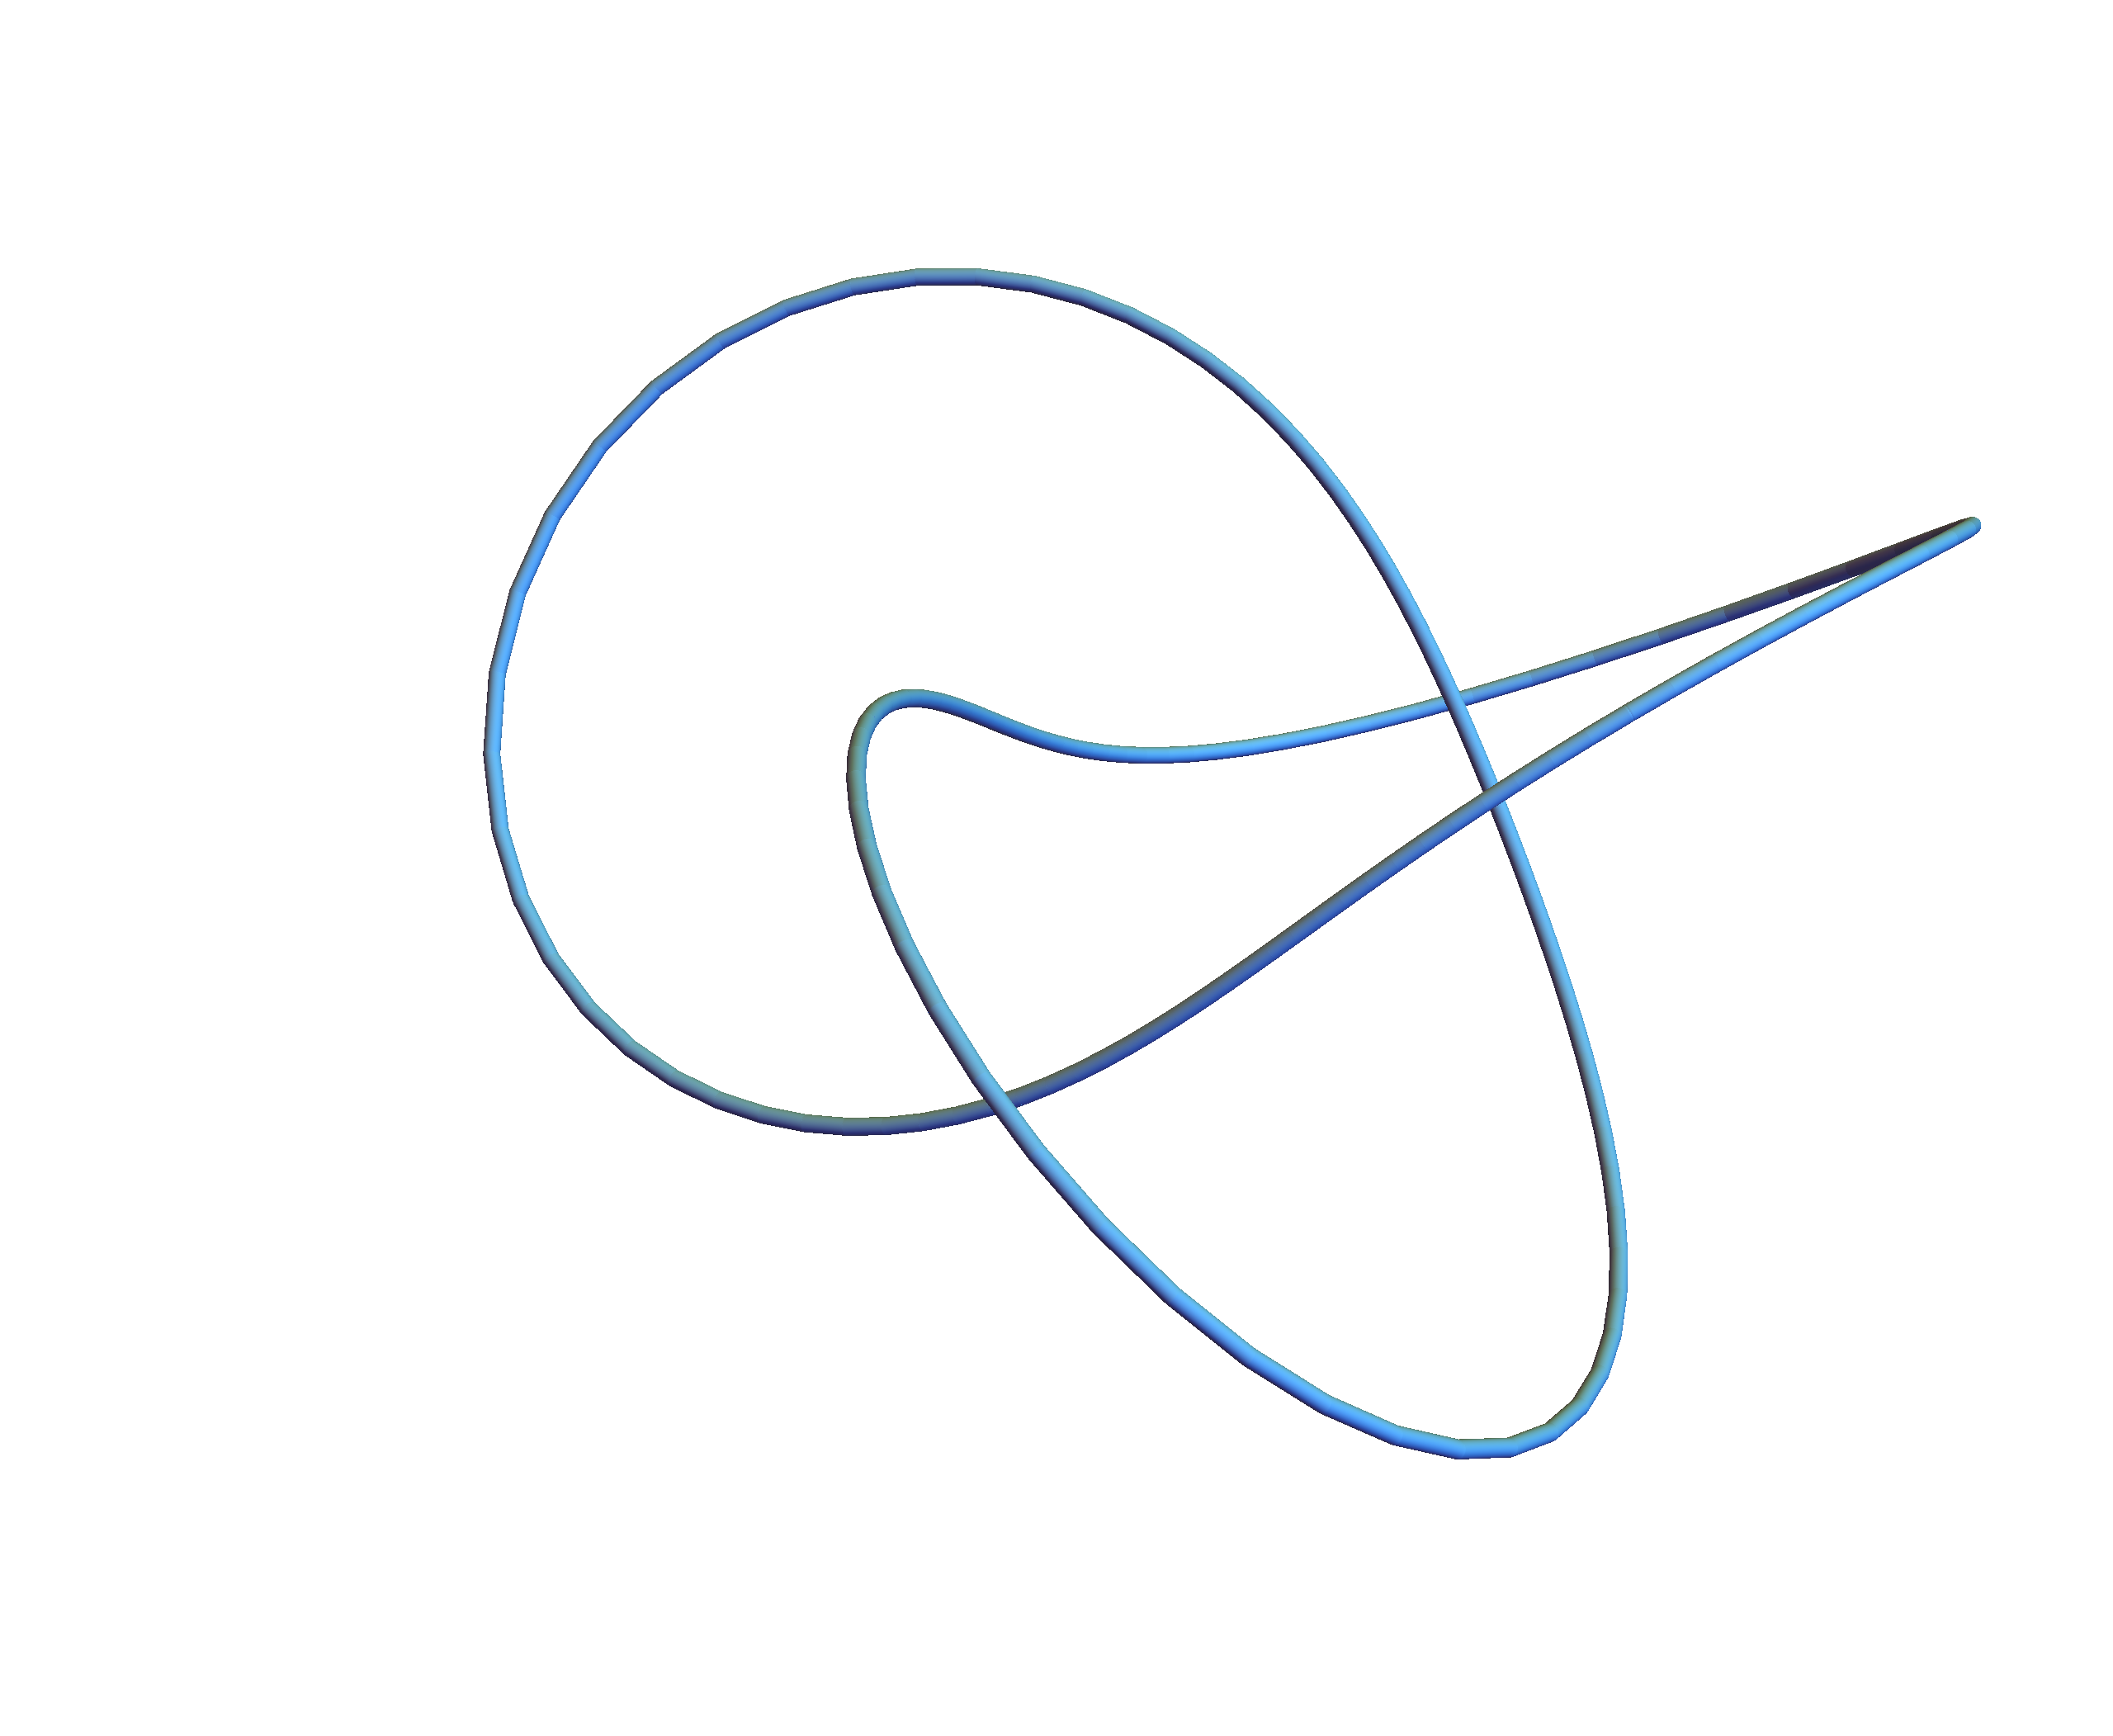
\includegraphics[width=0.5\linewidth]{figures/trefoil.png}
  \caption{A trefoil knot. While the knot is embedded inside $S^3$, we can stereographically project $S^3$ to $\R^3$ for visualization purposes.}
  \label{fig:trefoil}
\end{figure}

In our case, we're interested in a particular prototypical knot called the \defnphrase{trefoil} (visualized in Figure~\ref{fig:trefoil}).
This is the knot that, when laid on the surface of the torus, crosses the meridian of the torus three times and crosses longitudinal circles twice---as such it is also known as the \defnphrase{$(2, 3)$-torus knot}.

For any knot $K : S^1 \into S^3$, we can study the \defnphrase{knot complement} space $S^3 \wo K$.
Historically, such spaces have provided useful knot invariants via their fundamental group and interesting examples of 3-manifolds.
The fundamental group of the trefoil complement happens to be isomorphic to a famous group with a convenient physical interpretation, which we will describe shortly.
First, we recall the definition of a fundamental group as well as a useful theorem for computing fundamental groups.

\begin{defn}
  Let $X$ be a topological space. A \defnphrase{loop in $X$ based at $p$} is a continuous map $f : I \to X$ such that $f(0) = f(1) = p$.
  Two loops $f$ and $g$ based at $p$ are \defnphrase{path-homotopic} if there exists a continuous map $H : I \times I \to X$ such that for all $s$ and $t$ in $I$, $H(s, 0) = f(s)$,  $H(s, 1) = g(s)$, and $H(0, t) = H(1, t) = p$.
  The path-homotopy relation is an equivalence relation on the set of all loops in $X$ based at $p$, and we call the equivalence class of a loop its \defnphrase{path class}.
  The \defnphrase{fundamental group of $X$ based at $p$} is the set of path classes of loops in $X$ based at $p$, denoted $\pi_1(X, p)$.
  The set $\pi_1(X, p)$ forms a group under the operation of path composition.
\end{defn}

Morally, two loops in $X$ are homotopic if they can be continuously deformed into one another.
The fundamental group describes the group structure of all based loops in $X$ up to homotopy.

There is no general method for computing the fundamental group of an arbitrary topological space.
Instead, we rely on a toolkit of methods and theorems that prove useful in different situations.
One essential such tool is the Seifart Van-Kampen theorem.

\begin{defn}
  Let $H$, $G_1$, and $G_2$ be groups with presentations
  \begin{align*}
    G_1 &\cong \ang{\alpha_1, \dots, \alpha_m : \rho_1, \dots, \rho_r}, \\
    G_2 &\cong \ang{\beta_1, \ldots, \beta_n : \sigma_1, \ldots, \sigma_s}, \text{ and } \\
    H &\cong \ang{\gamma_1, \ldots, \gamma_p : \tau_1, \ldots, \tau_t}.
  \end{align*}
  Then if $f_1 : H \to G_1$ and $f_2 : H \to G_2$ are group homomorphisms, the \defnphrase{amalgamated free product} of $G_1$ and $G_2$ along $H$ is the group with presentation
  \begin{align*}
    G_1 \ast_H G_2 \cong \ang{&\alpha_1, \ldots \alpha_m,\, \beta_1, \ldots, \beta_n : \rho_1, \ldots, \rho_r, \\
    &\sigma_1, \ldots, \sigma_s,\, u_1 = v_1,\ldots, u_p = v_p}
  \end{align*}
  where $u_a$ is an expression for $f_1(\gamma_a) \in G_1$ in terms of the generators $\{\alpha_i\}$ and $v_a$ similarly expresses $f_2(\gamma_a) \in G_2$ in terms of $\{\beta_j\}$.
\end{defn}

\begin{thm}[Seifert-van Kampen Theorem]
  Let $X$ be a topological space, and suppose that $X = U_1 \cup U_2$ for two open and path-connected subsets $U_1,\ U_2 \subseteq X$. 
  In addition, suppose that $U_1 \cap U_2$ is path-connected and nonempty, and let $p \in U_1 \cap U_2$.
  There exists an isomorphism
  \begin{equation*}
    \Phi : \pi_1(U_1, p) \ast_{\pi_1(U_1 \cap U_2,\, p)} \pi_2(U_2, p) \to \pi_1(X, p)
  \end{equation*}
  such that the following diagram commutes:
  \begin{center}
    \begin{tikzcd}
      & \pi_1(U_1) \ar[dr, bend left=20, "j_1",] \ar[d, hookrightarrow] & \\
      \pi_1(U_1 \cap U_2) \ar[ur, bend left=20, "i_1"] \ar[dr, bend right=20, "i_2"'] & \pi_1(U_1) \ast_{\pi_1(U_1 \cap U_2)} \pi_2(U_2) \ar[r, "\Phi", dashed] \ar[d, hookleftarrow] & \pi_1(X) \\
      & \pi_1(U_2) \ar[ur, bend right=20, "j_2"'] & 
    \end{tikzcd}
  \end{center}
\end{thm}

Now, we provide an explicit computation of the fundamental group of the trefoil complement.
For additional details, see~\cite[47--49]{hatcher2002} and~\cite[153--154]{stillwell1993}.

\begin{prop}
  Let $K$ be the trefoil knot.
  Then
  \begin{equation*}
    \pi_1(S^3 \wo K) = \ang{x, y : x^2 = y^3}
  \end{equation*}
\end{prop}

\begin{proof}
  We proceed by two applications of the Seifert-van Kampen theorem.
  First we compute $\pi_1(\R^3 \wo K)$, since it is slightly easier to compute than $\pi_1(S^3 \wo K)$.

  Let $T \subset \R^3 \wo K$ be the solid torus with $K$ removed and $N$ be a thin tubular neighborhood of $K$.
  Let $X = T \wo N$ and $Y = (\R^3 \wo T) \wo N$.
  Then $X$ and $Y$ meet at a region $L$ that looks like the surface of the solid torus with $N$ removed.
  As shown in Figure~\ref{fig:flat_annulus}, $L$ is an annulus.

  \begin{figure}[h]
    \centering
    \includegraphics[width=0.7\textwidth]{figures/fundamental_group_flat.pdf}
    \caption{The region $L$ is the torus with a thin tubular neighborhood of the trefoil $N$ removed. Here, $N$ is depicted in white and $L$ is shaded in gray on the flat torus. While still respecting the appropriate edge identifications, the pieces of the torus can be rearranged to form an annulus. The generator $\ell$ of $\pi_1$ of this annulus is shown in blue.}
    \label{fig:flat_annulus}
  \end{figure}

  Since $L$ is an annulus, its fundamental group is infinite cyclic with a single generator $\ell$.
  The space $X$ is a solid torus with a neighborhood of the trefoil removed, which deformation retracts onto a circle.
  So $\pi_1(X)$ is infinite cyclic as well, with generator $x$ corresponding to the loop around the axis of the solid torus.
  In $X$, the generator $\ell$ is a trefoil loop around the torus that crosses longitudinal circles twice, so we have
  \begin{equation*}
    \ell \simeq x^2.
  \end{equation*}
  The fundamental group of $Y$ is also infinite cyclic, with the generator $y$ corresponding to a loop that ``links'' the hole of the solid torus.
  The loop $\ell$ crosses meridian circles in the solid torus three times, so we have that
  \begin{equation*}
    \ell \simeq y^3.
  \end{equation*}
  Now, we can expand $X$ and $Y$ slightly to open sets $X' \supseteq X$ and $Y' \supseteq Y$ such that $X' \cap Y'$ is an open neighborhood of $L$ and $X' \cup Y' = \R^3 \wo K$ (see Figure~\ref{fig:fundamental_group_side}).
  Then, applying Van Kampen, we have that
  \begin{equation*}
    \pi_1(\R^3 \wo K) = \ang{x, y : x^2 = y^3}.
  \end{equation*}

  \begin{figure}[t]
    \centering
    \includegraphics[width=0.6\textwidth]{figures/fundamental_group_side.pdf}
    \caption{The picture on the left shows a longitudinal slice of the torus $T$, with the absence of tubular neighborhood $N$ of the trefoil shown in white. The regions $X$ and $Y$ are depicted in blue and pink, respectively. On the right, $X$ and $Y$ have been expanded to $X'$ and $Y'$, respectively.}
    \label{fig:fundamental_group_side}
  \end{figure}

  Now we show that $\pi_1(\R^3 \wo K) = \pi_1(S^3 \wo K)$ with another application of Van Kampen.
  Decompose $S^3 \wo K$ into $(\R^3 \wo K) \cup B$, where $B$ is an open set containing the compactification point and the complement of a large closed ball containing $K$.
  Both $B$ and $B \cap (\R^3 \wo K)$ are simply connected.
  By Van Kampen, the inclusion $\R^3 \wo K \into S^3 - K$ induces an isomorphism of groups
  \begin{equation*}
    \Phi : \pi_1(R^3 \wo K,) \to \pi_1(S^3 \wo K)
  \end{equation*}
  as shown by the following commutative diagram:
  \begin{center}
    \begin{tikzcd}
      & \pi_1(\R^3 \wo K) \ar[dr, bend left=20] \ar[d, hookrightarrow] & \\
      \pi_1(B \cap (\R^3 \wo K)) \ar[ur, bend left=20] \ar[dr, bend right=20, "1"'] & \pi_1(B) \ast \pi_1(\R^3 \wo K) \ar[r, "\Phi", dashed] \ar[d, hookleftarrow] & \pi_1(S^3 \wo K) \\
      & \pi_1(B) \ar[ur, bend right=20, "1"'] & 
    \end{tikzcd}
  \end{center}
  Thus we have the desired result.
\end{proof}

The fundamental group of the trefoil complement is isomorphic to a well-known group, the \defnphrase{braid group on $3$ strands}.
This group has presentation
\begin{equation*}
  B_3 = \ang{\sigma_1, \sigma_2 : \sigma_1 \sigma_2 \sigma_1 = \sigma_2 \sigma_1 \sigma_2}.
\end{equation*}
The isomorphism $\pi_1(S^3 \wo K) \to B_3$ is given by sending generators
\begin{equation}\label{eq:iso_pi1_b3}
  \begin{aligned}
    x &\mapsto \sigma_0 \sigma_1 \sigma_0 \\
    y &\mapsto \sigma_0 \sigma_1
  \end{aligned}
\end{equation}
This group appears in many different contexts: it is the mapping class group of the thrice-punctured disk, the universal central extension of $\PSLZ$, and so forth.
It also has a convenient visual interpretation, where the generators $\sigma_1$ and $\sigma_2$ are depicted and composed as in Figure~\ref{fig:visual_braid_group}.
We will return to this visual interpretation in Chapter~\ref{chap:finite_subsets}, where we decompose the path class of various loops in $\exptwothree S^1 \cong S^3 \wo K$ as visual generators of $B_3$. 

\vspace{1em}
\begin{figure}[h]
  \centering
  \begin{subfigure}[t]{0.48\textwidth}
    \centering
    \begin{tikzpicture}
      \braid[ultra thick, number of strands=3, width=5mm, height=21mm] s_1;
    \end{tikzpicture}
    \hspace{10mm}
    \begin{tikzpicture}
      \braid[ultra thick, number of strands=3, width=5mm, height=21mm] s_2;
    \end{tikzpicture}
    \caption{The generators $\sigma_1$ and $\sigma_2$ of $B_3$}
  \end{subfigure}
  \hfill
  \begin{subfigure}[t]{0.48\textwidth}
    \centering
    \begin{tikzpicture}
      \braid[ultra thick, width=5mm, height=7mm, style strands={2}{strand}] s_1 s_2 s_1;
      \draw node[fill=white] at (2,-1.25) {=};
    \end{tikzpicture}
    \begin{tikzpicture}
      \braid[ultra thick, width=5mm, height=7mm, style strands={2}{strand}] s_2 s_1 s_2;
    \end{tikzpicture}
    \caption{The single relation in $B_3$, known as the \textbf{third Reidmeister move}.}
  \end{subfigure}
  \caption{The visual interpretation of $B_3$, where each generator is thought of as a braiding of three strands of string that start and end at fixed points. The group operation corresponds to stacking the visual generators top to bottom to compose a more complex braiding of string. The single relation in $B_3$ can be thought of as ``pulling a string'' without moving the endpoints, which preserves the isotopy class of the braid.}
  \label{fig:visual_braid_group}
\end{figure}

\section{From $\LS$ to $S^3$}\label{sec:lattice_to_s3}

At first glance, the space of two-dimensional lattices up to homothety and the three-dimensional sphere may seem quite different.
It turns out that they are indeed homeomorphic.
We now describe an explicit homeomorphism $\LS \to S^3$ as sketched by Mostovoy in~\cite{mostovoy2004}.

Let $L \in \LS$ and $k \in \Z$.
Define
\begin{equation*}
  G_k(L) = \sum_{\omega \in L,\ \omega \neq 0} \omega^{-k}.
\end{equation*}
When $k \geq 4$, this series converges and is known as an \defnphrase{Eisenstein series}.
For nondegenerate $L$, these numbers are the parameters in the Weierstrass $\wp_L$-function identity
\begin{equation*}
  (\wp_L')^2 = 4 \wp_L^3 - 60 G_4(L) \wp_L - 140 G_6(L).
\end{equation*}
The following facts about $G_4(L)$ and $G_6(L)$ are fundamental to the theory of elliptic functions:
\begin{enumerate}[(i)]
  \item For $t > 0$ and any $L$, $G_4(tL) = t^{-4} G_4(L)$ and $G_6(tL) = t^{-6} G_6(L)$~\cite[631]{abramowitz1964}
  
  \item The map $L \mapsto (G_4(L),\, G_6(L))$ is a homeomorphism $\LS \to \C^2 \wo \{ 0 \}$~\cite[82, 89]{serre1973}.

  \item A tuple $(u, v) \in \C^2 \wo \{ 0 \}$ is the image of a degenerate lattice under this map if and only if $20u^3 - 49v^2 = 0$~\cite[265]{ghys2007}.
\end{enumerate}
Thus for any nontrivial lattice $L$, we can obtain a unique rescaling $L' = tL$ for some $t > 0$ such that
\begin{equation*}
  |G_4(L')|^2 + |G_6(L')|^2 = 1
\end{equation*}
Then the map $L \mapsto (G_4(L'),\, G_6(L'))$ lands in $S^3$, and we have the desired homeomorphism $\LS \to S^3$.

The image of the degenerate lattices under this map is the intersection of the curve $20u^3 - 49v^2 = 0$ with the 3-sphere. For any $a \in \R$, it happens that the intersection of complex curve $u^3 + av^2 = 0$ with the 3-sphere is a trefoil knot \cite[4]{milnor1968}. Thus, the image of degenerate lattices under the homeomorphism is the trefoil shown in Figure~\ref{fig:trefoil}.

\section{The linking number of periodic orbits in $S^3$}\label{sec:periodic_orbits_in_s3}

We have observed the periodic orbits of the modular flow in the space of lattices in Section~\ref{subsec:lattice_flow}, and we have just seen that the space of lattices is homeomorphic to the 3-sphere.
It is now natural to ask: how do these periodic orbits present in the 3-sphere?

The degenerate lattices are sent to the trefoil knot in the 3-sphere, but the periodic orbits of this flow exist entirely within the space of nondegenerate lattices.
Thus we can say that in the 3-sphere, a periodic orbit of the modular flow in the space of lattices determines a link with the trefoil knot.
Since each periodic flow is associated with some hyperbolic $A \in \SLZ$ we call the corresponding trefoil link $k_A$ a \defnphrase{modular trefoil link} or \defnphrase{modular knot}, following after~\cite{ghys2007}.
Several examples of such links are shown in Figure~\ref{fig:trefoil_links}.

\begin{figure}[h!]
  \centering
  \begin{subfigure}[t]{0.48\textwidth}
    \centering
    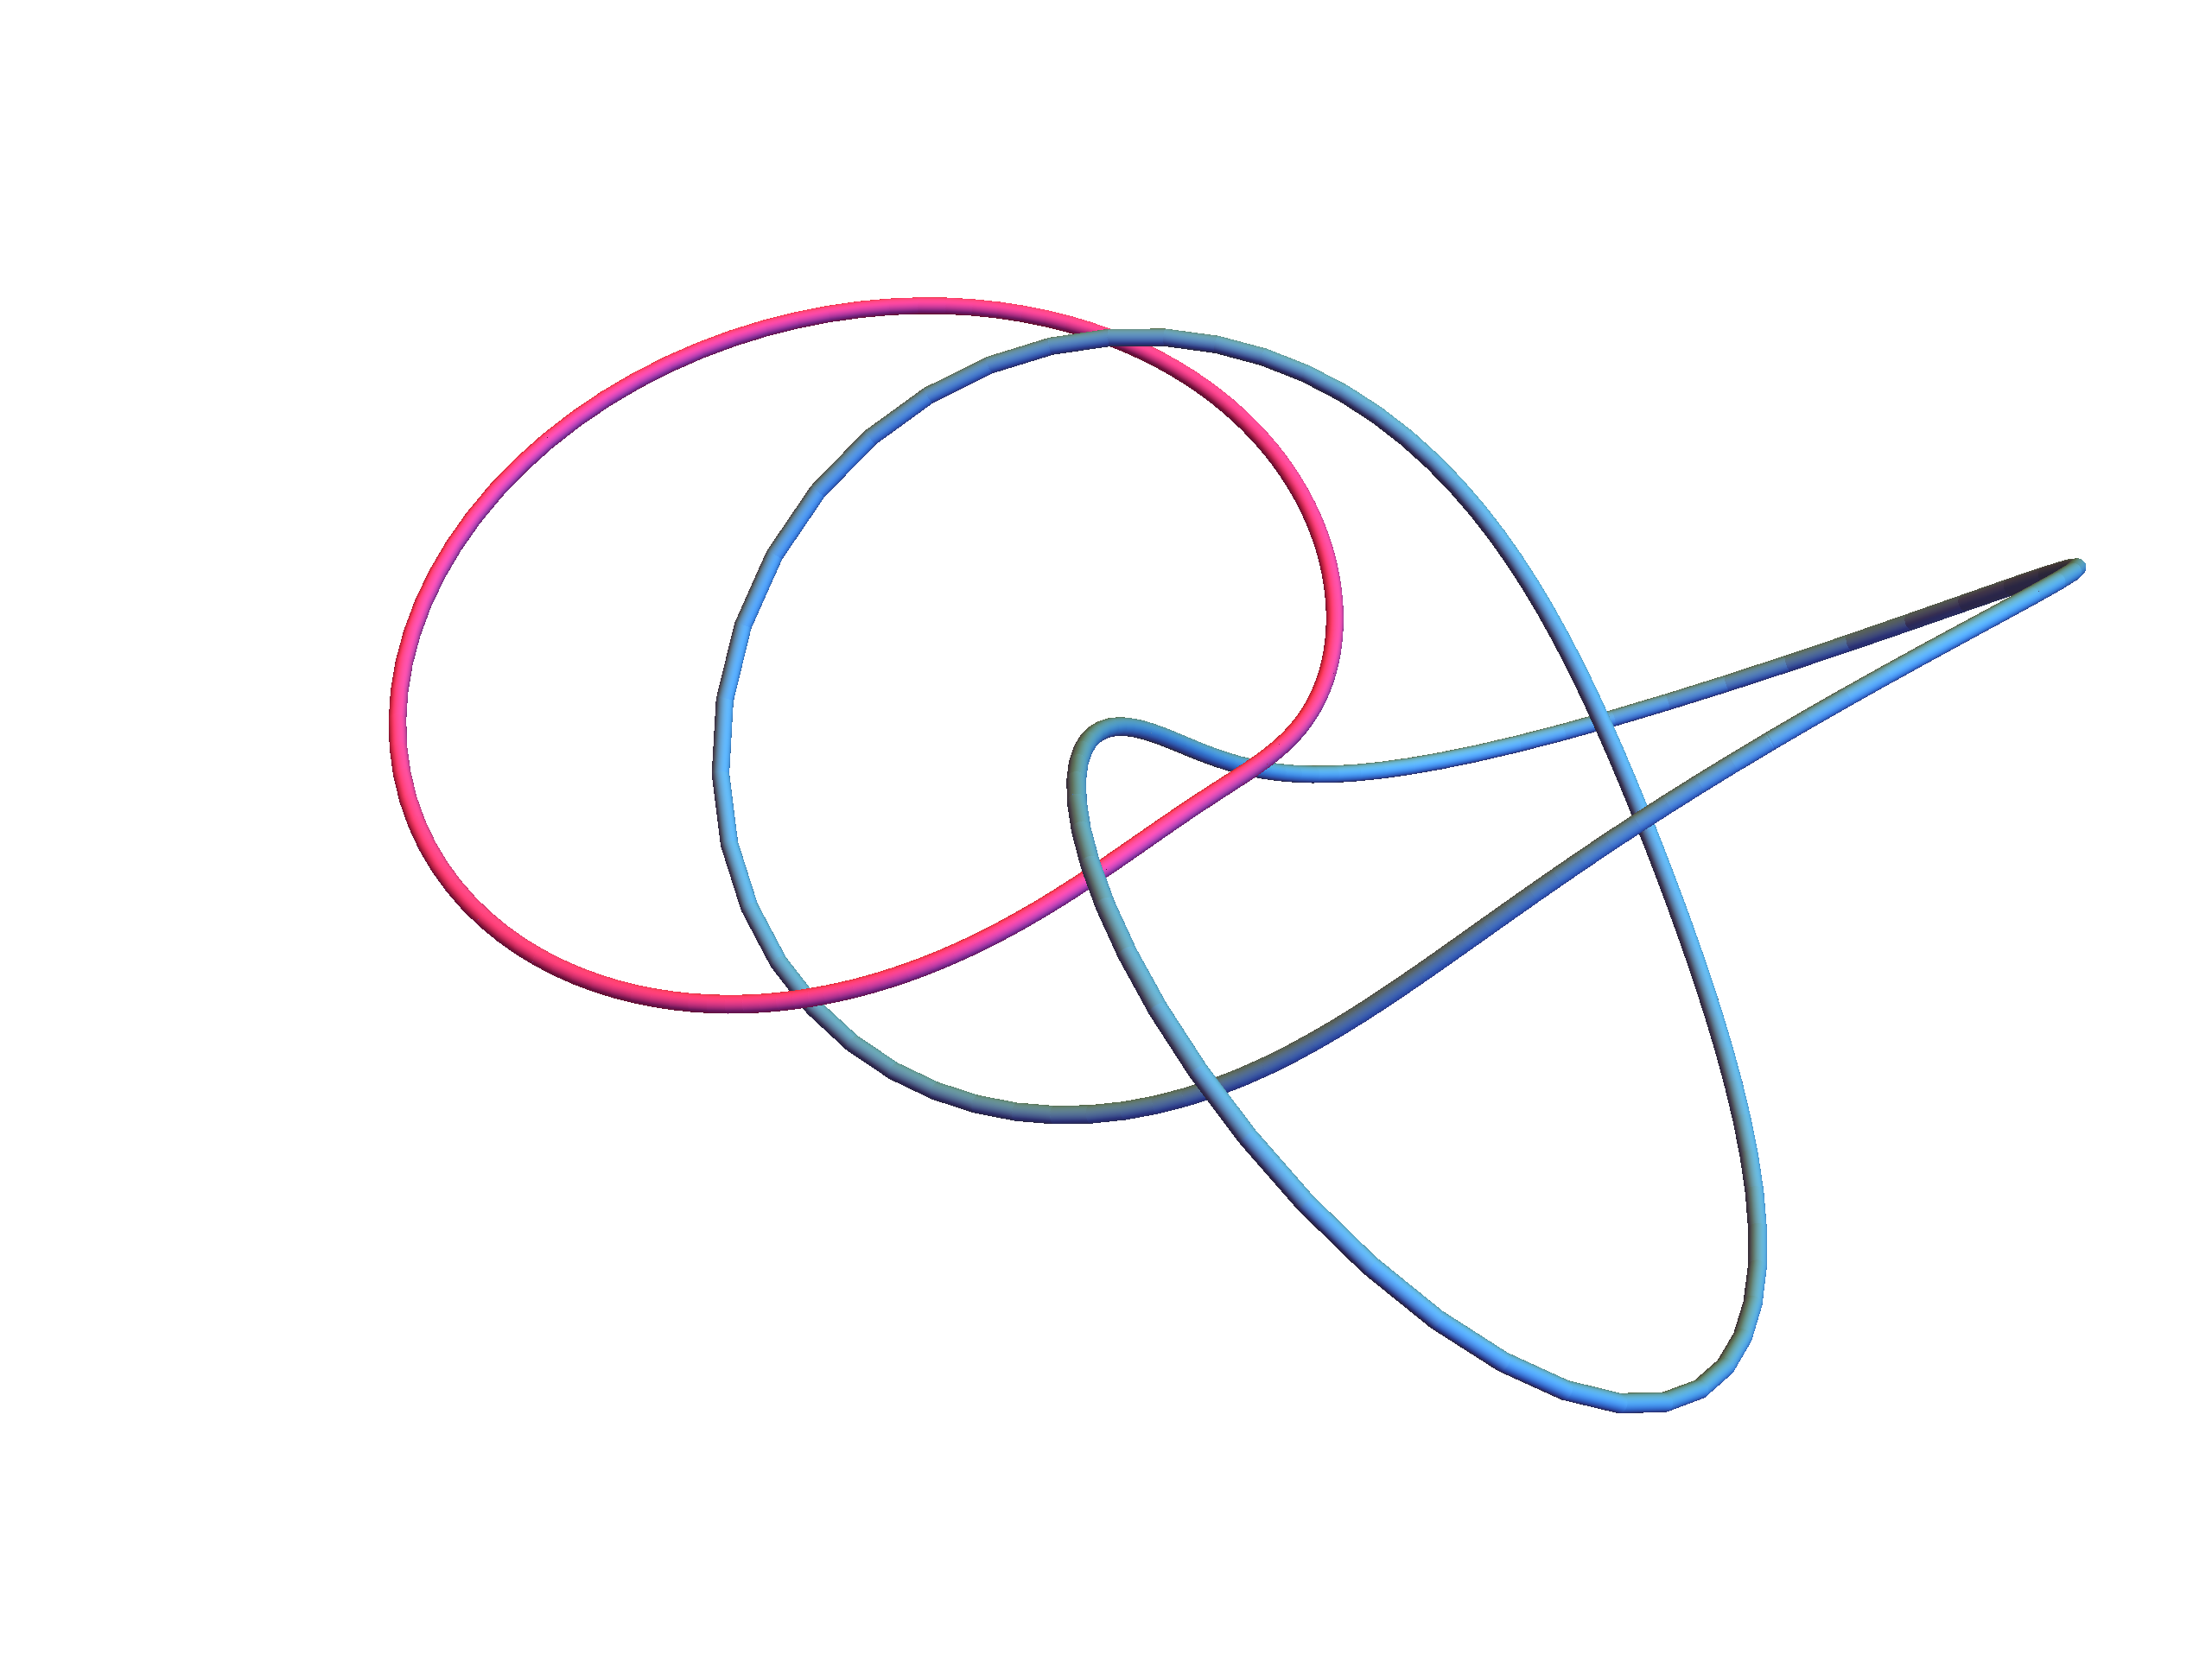
\includegraphics[width=\textwidth]{figures/trefoil_link_1_1_1_2.png}
    \caption*{$A = \begin{pmatrix}1 & 1 \\ 1 & 2\end{pmatrix}$}
  \end{subfigure}
  \hfill
  \begin{subfigure}[t]{0.48\textwidth}
    \centering
    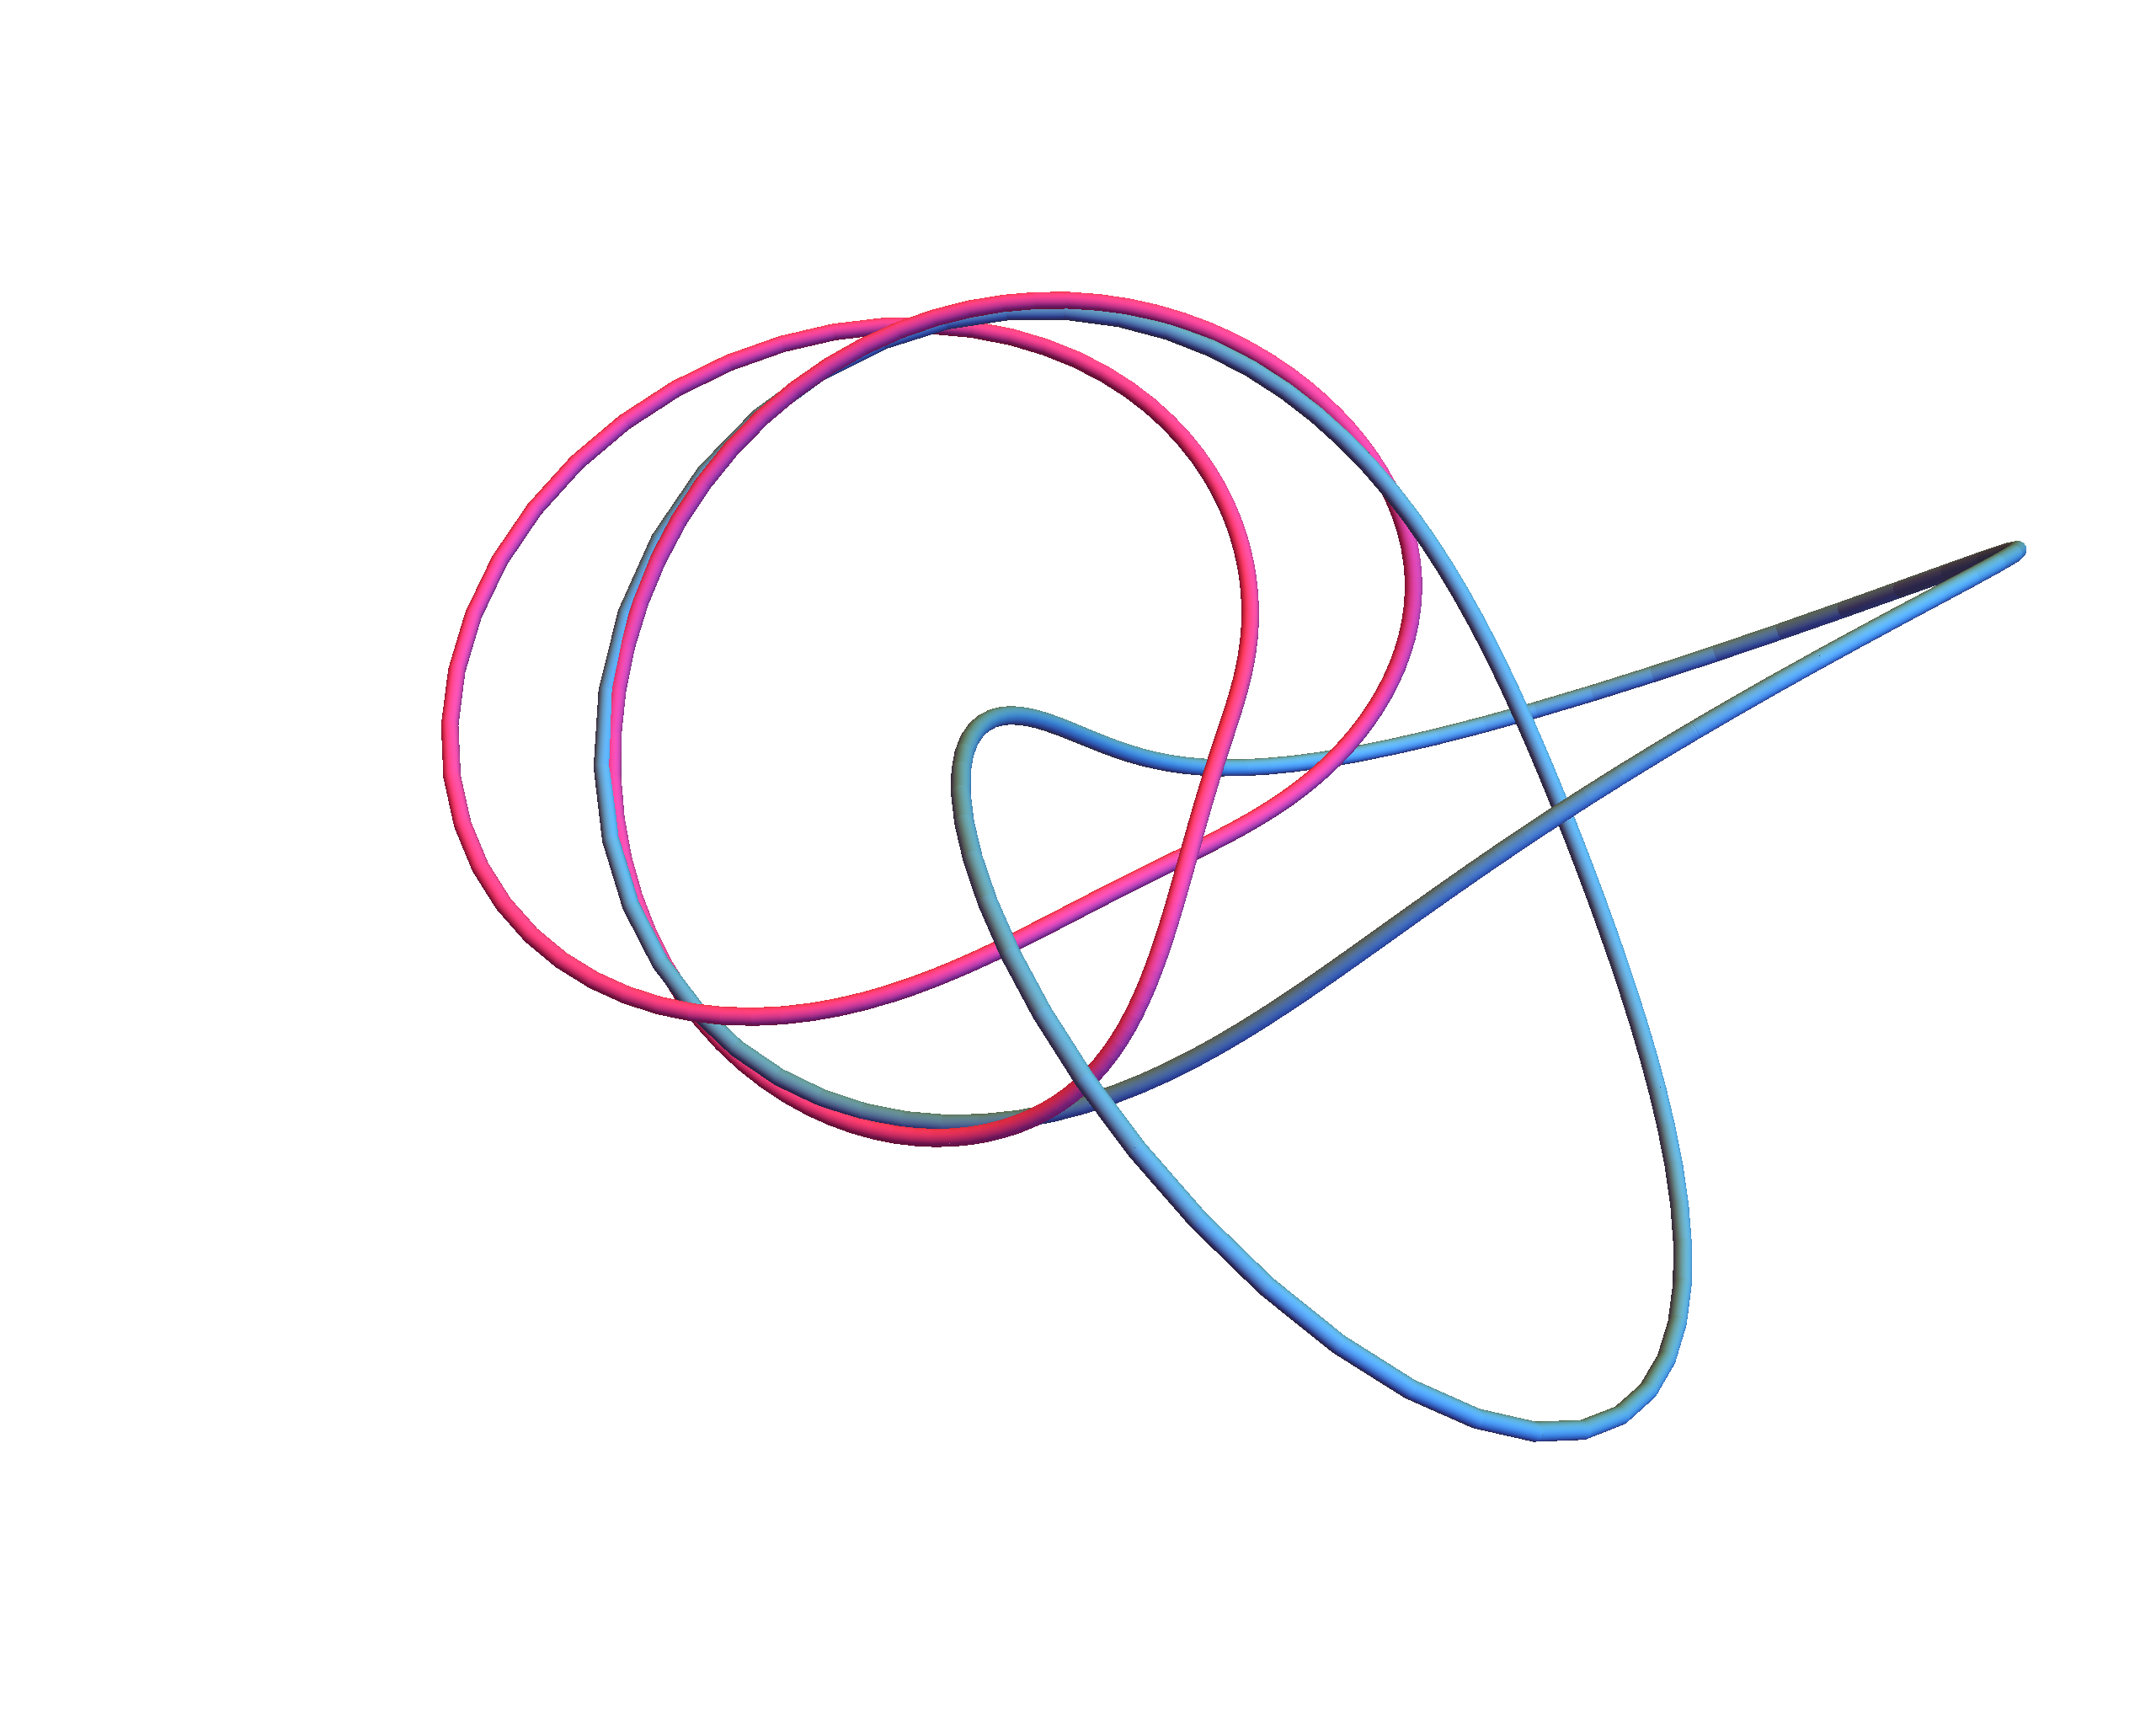
\includegraphics[width=\textwidth]{figures/trefoil_link_2_3_5_8.png}
    \caption*{$A = \begin{pmatrix}2 & 3 \\ 5 & 8\end{pmatrix}$}
  \end{subfigure}
  \begin{subfigure}[t]{0.48\textwidth}
    \centering
    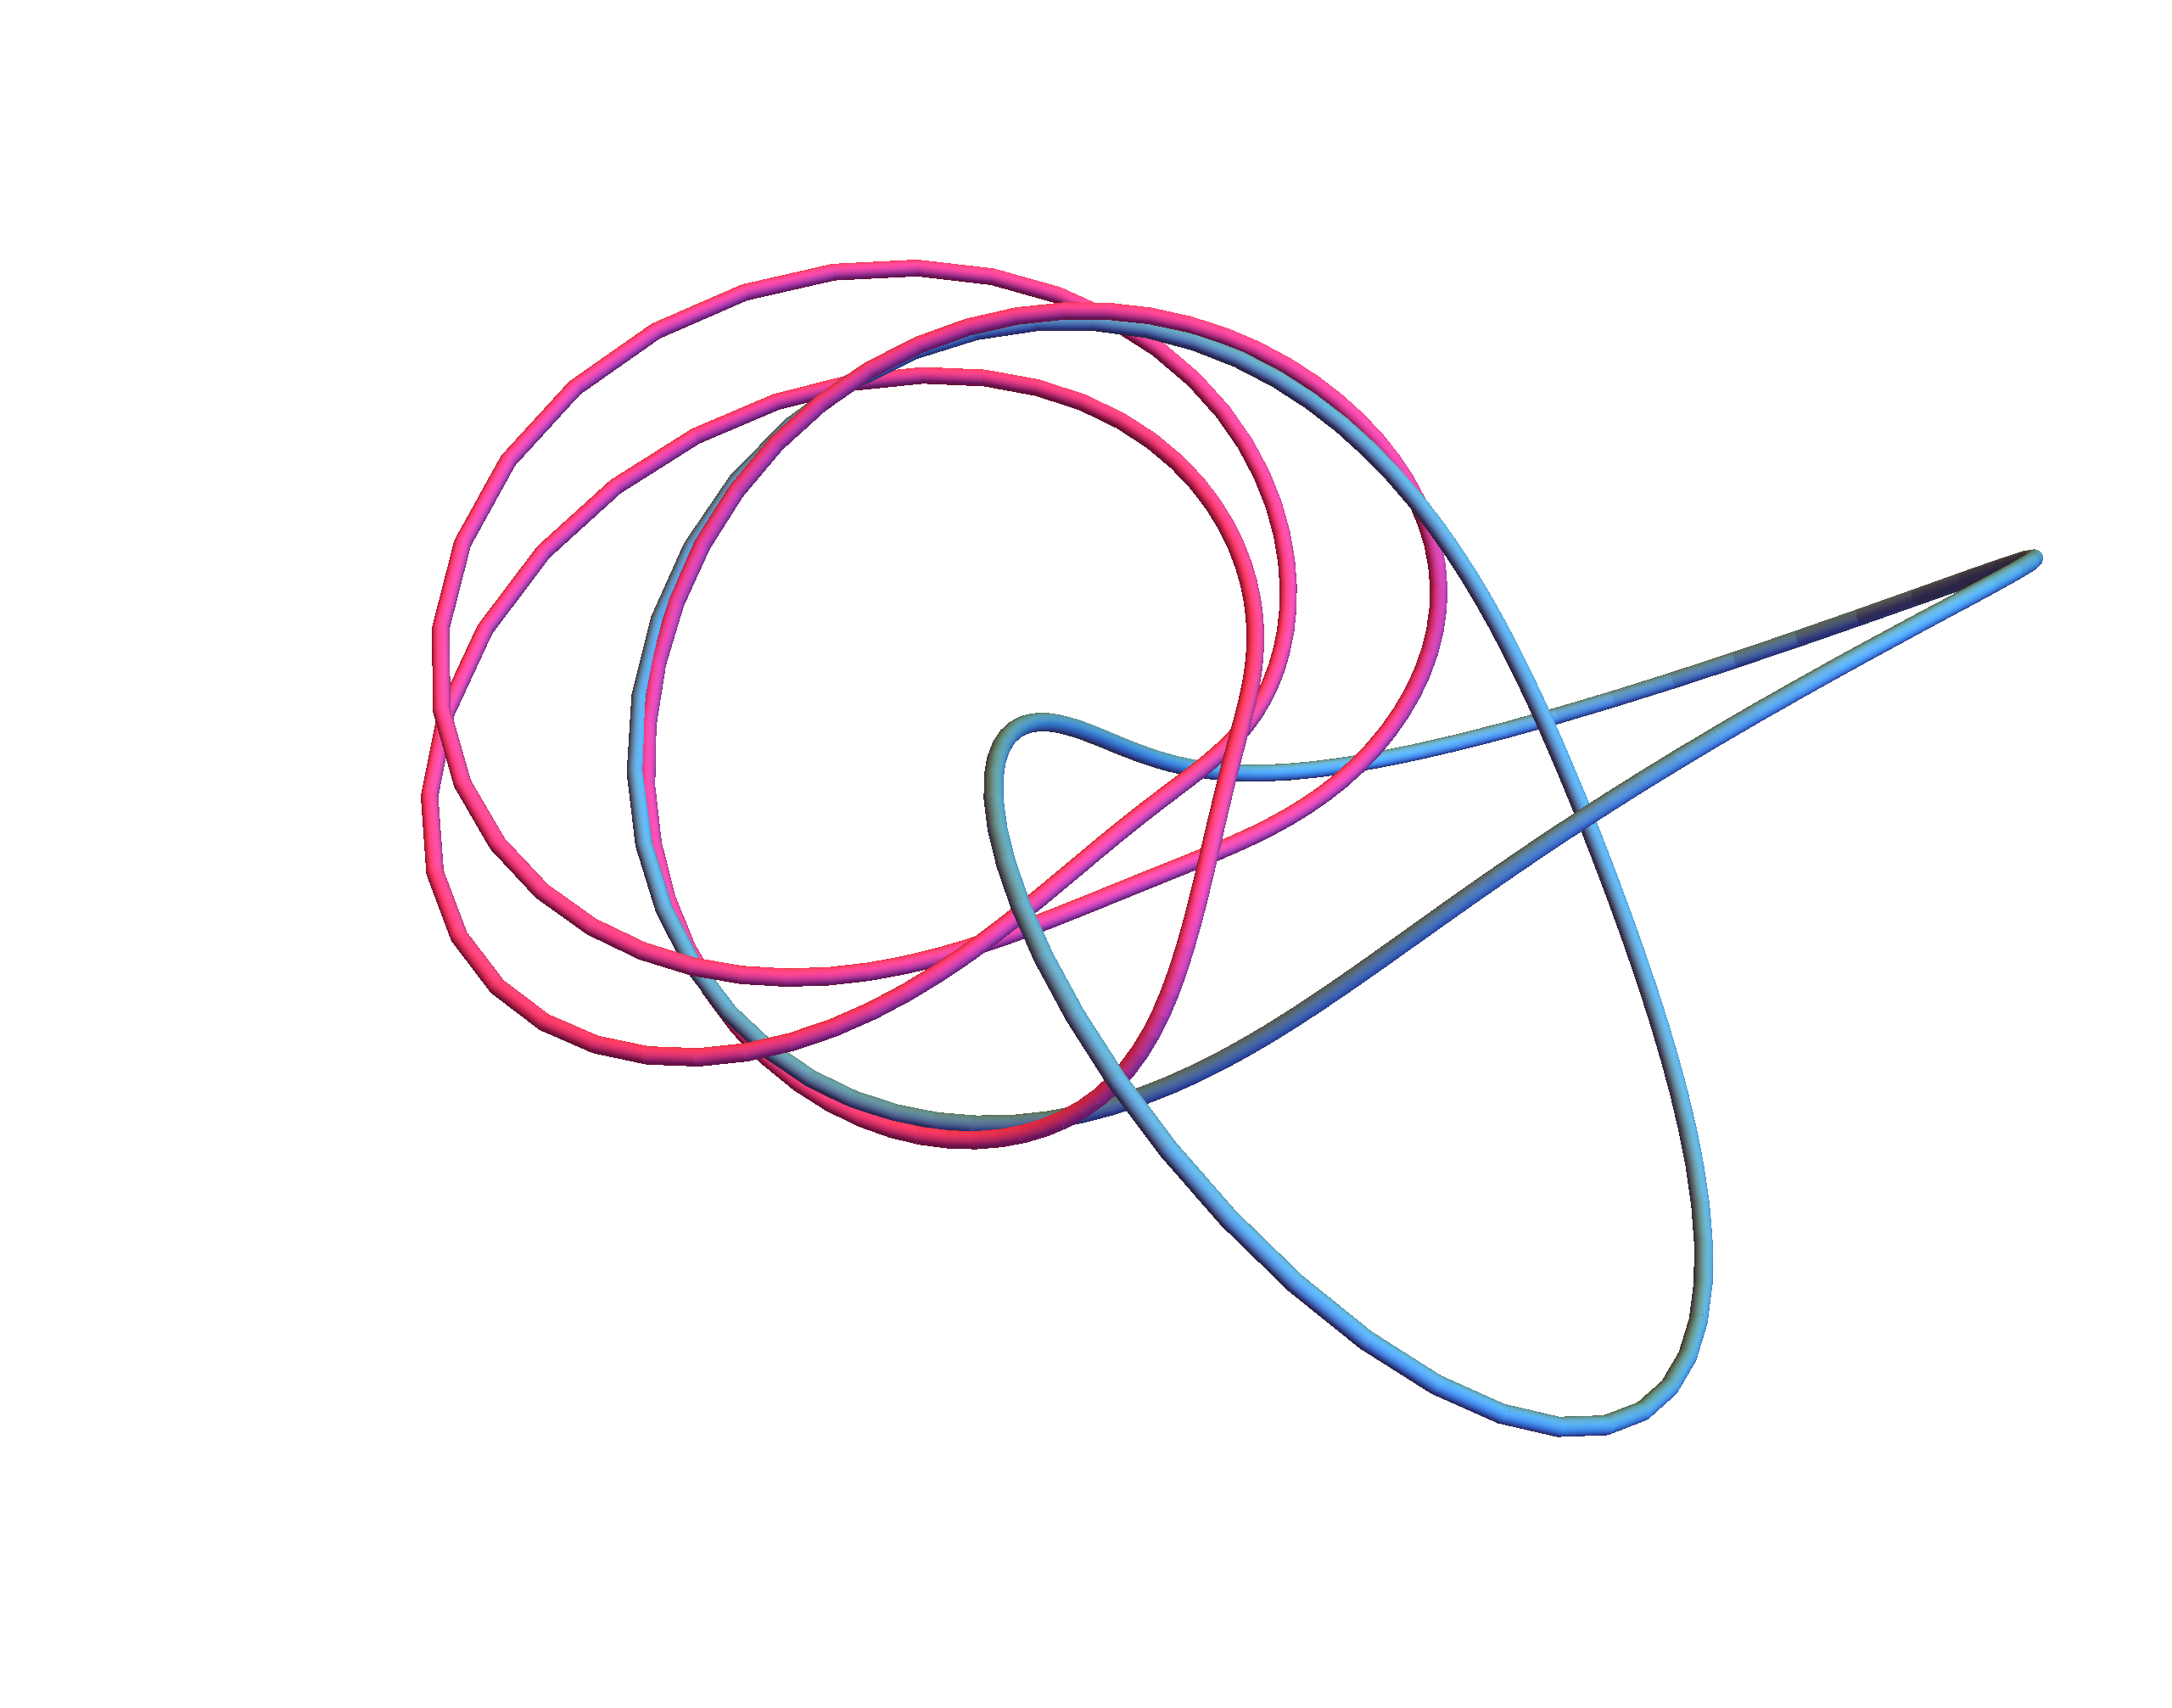
\includegraphics[width=\textwidth]{figures/trefoil_link_13_8_21_13.png}
    \caption*{$A = \begin{pmatrix}13 & 8 \\ 21 & 13\end{pmatrix}$}
  \end{subfigure}
  \hfill
  \begin{subfigure}[t]{0.48\textwidth}
    \centering
    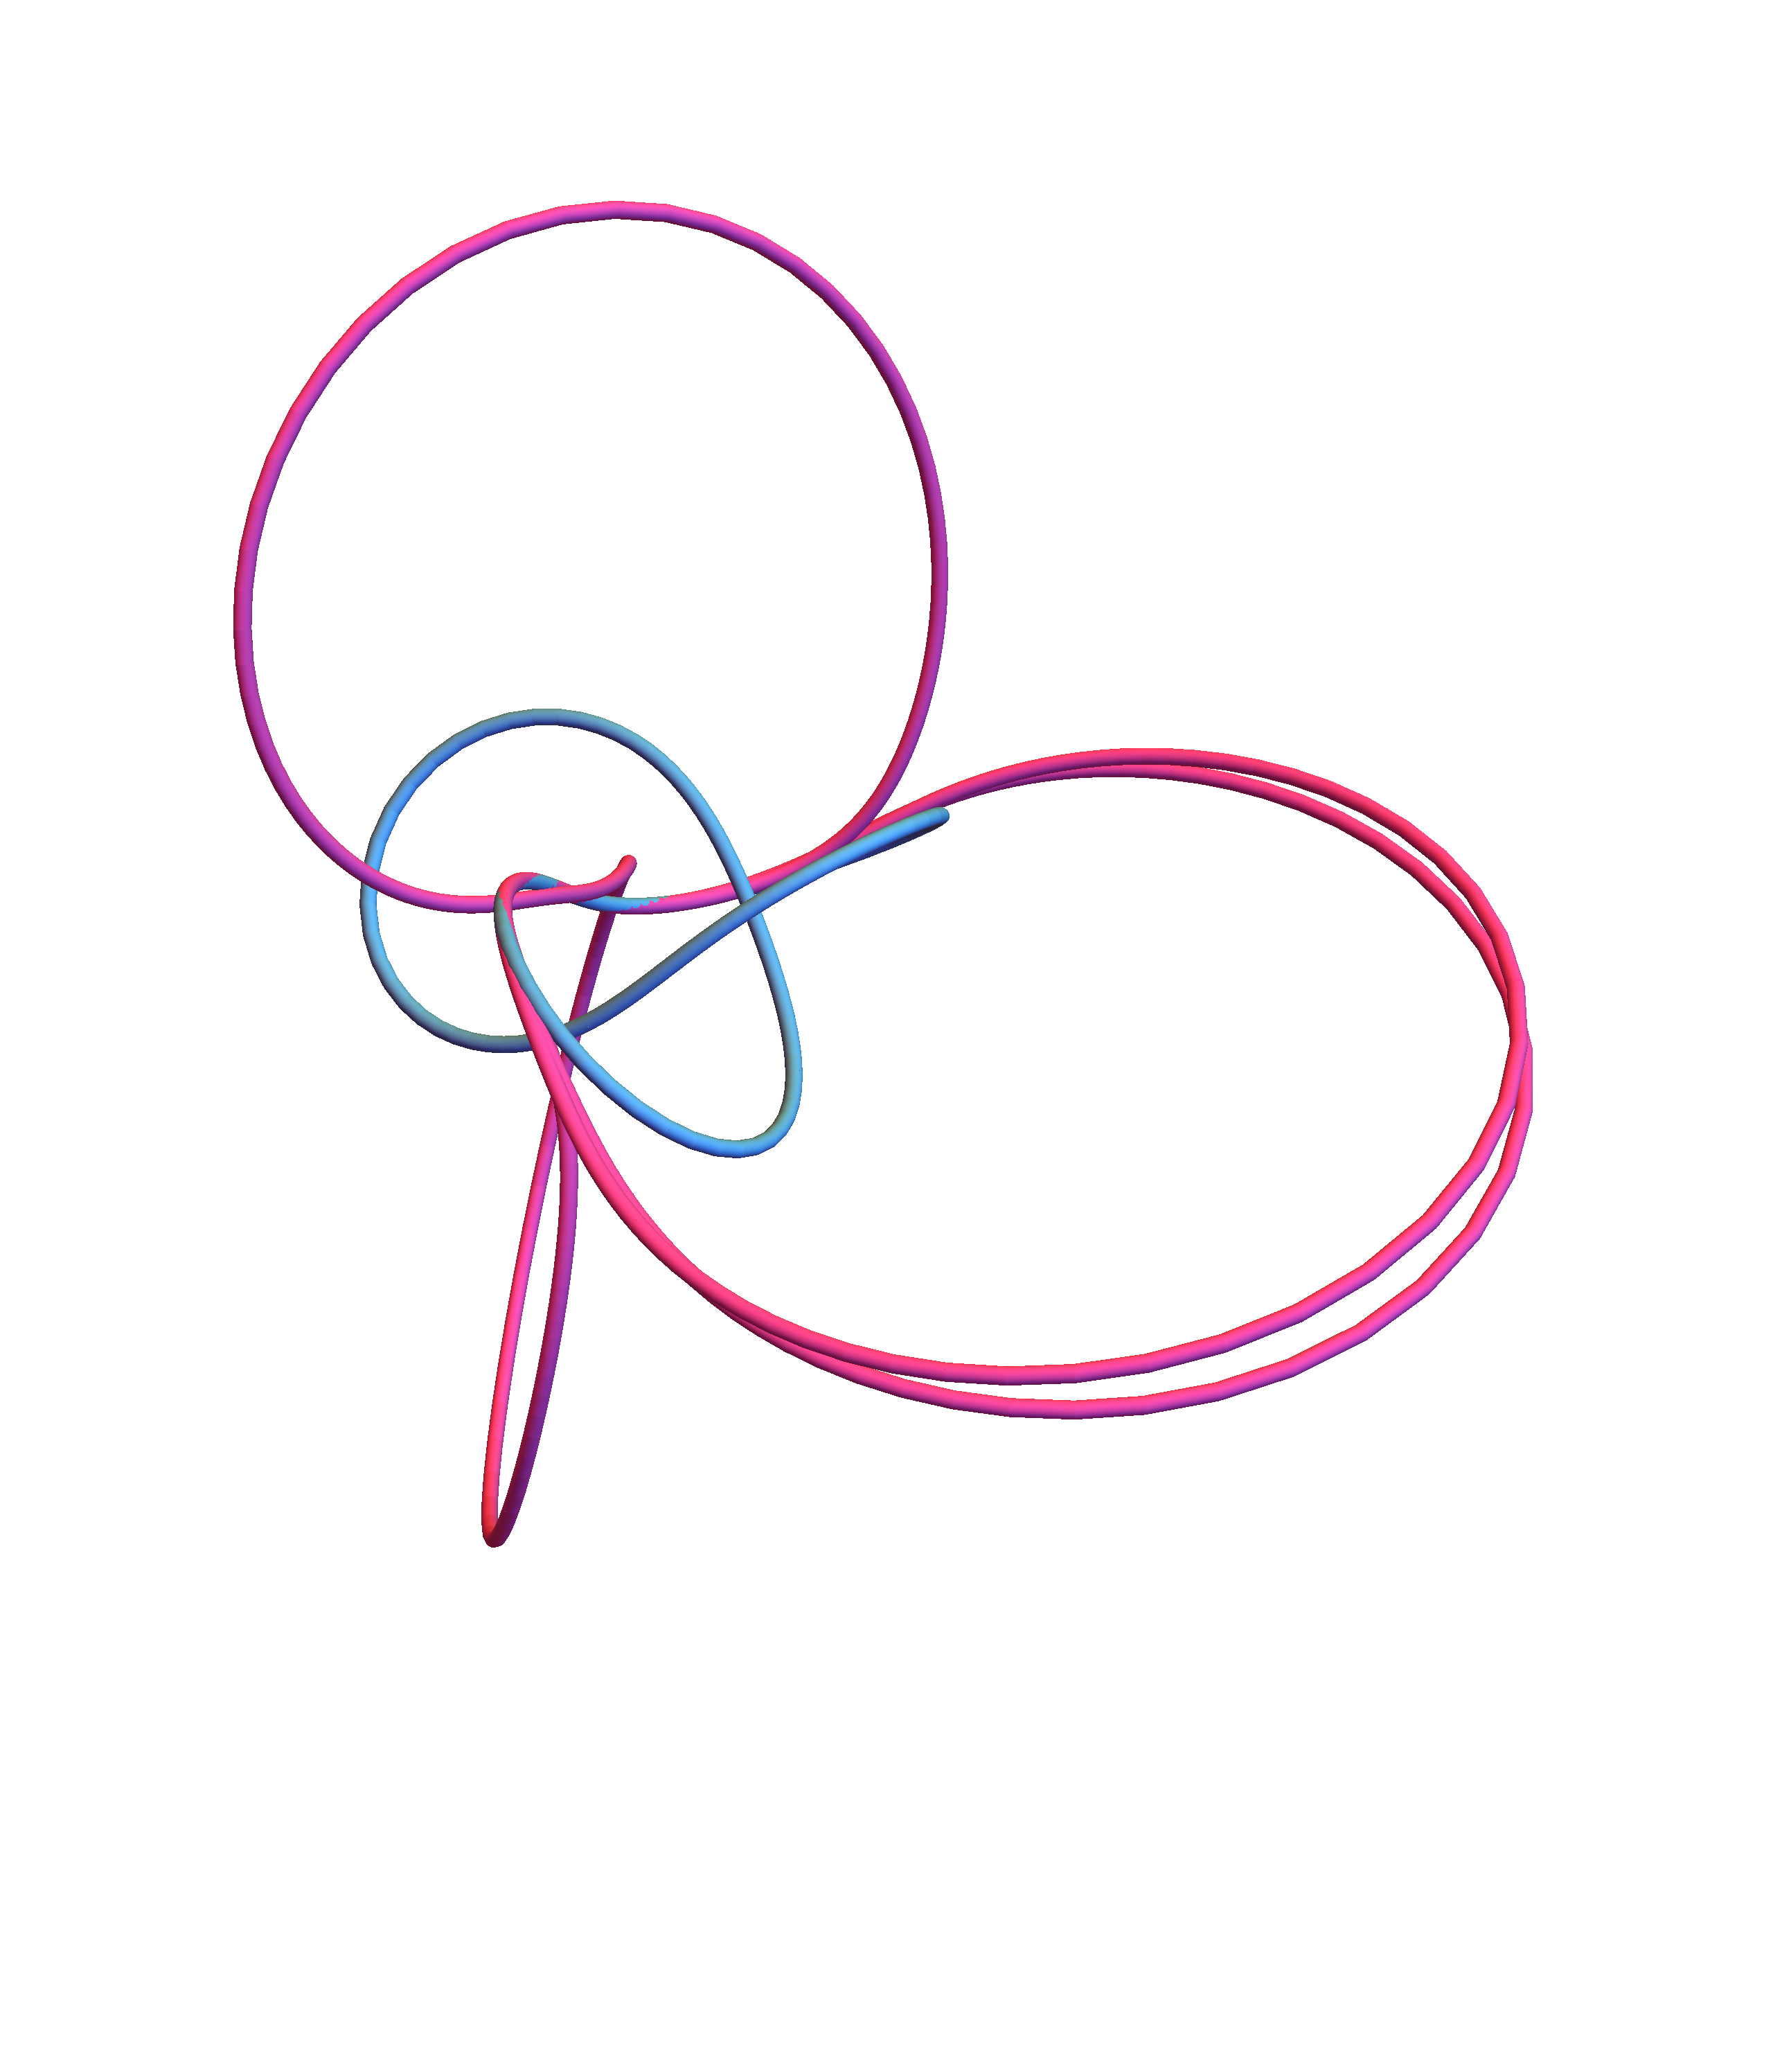
\includegraphics[width=\textwidth]{figures/trefoil_link_43_163_67_254.png}
    \caption*{$A = \begin{pmatrix}43 & 163\\ 67 & 254\end{pmatrix}$}
  \end{subfigure}
  \caption{A matrix $A \in \SLZ$ determines a periodic orbit of a flow in $\LS$, which in turn determines a modular trefoil link $k_A$ in $S^3$. Here, we visualize $k_A$ for several values of $A$.}
  \label{fig:trefoil_links}
\end{figure}

The periodic orbits of the modular flow provide a rich variety of trefoil links.
One classically studied invariant of two-component links is their \defnphrase{linking number}, an integer associated with a particular link. The linking number of a two-component link can be defined computationally as follows:

\begin{enumerate}
  \item Color the components of the link red and blue, respectively, and give each component an orientation.
  \item Project the colored, oriented link onto the plane. Any regular projection will do.
  \item Assign each crossing of a red strand over blue strand a number, either $1$ or $-1$ according to the diagram in Figure~\ref{fig:linking_number}.
  \item Sum the integers at all crossings to obtain the linking number.
\end{enumerate}

\begin{figure}[t]
  \centering
  \includegraphics[width=0.3\linewidth]{figures/linking_number.pdf}
  \caption{Diagrammatic rules for computing the linking number of link.}
  \label{fig:linking_number}
\end{figure}

\begin{figure}[b]
  \centering
  \includegraphics[width=0.3\linewidth]{figures/linking_number_example.pdf}
  \caption{A simple link. The red component crosses over the blue component exactly once. According to Figure~\ref{fig:linking_number}, this link has linking number 1.}
  \label{fig:linking_number_example}
\end{figure}

A simple example is shown in Figure~\ref{fig:linking_number_example}.
For a more complex example, consider the first link in Figure~\ref{fig:trefoil_links}; it has linking number 0.

In \cite{ghys2007}, Ghys proves a fascinating result relating the linking numbers of modular trefoil links to a famous arithmetic function.
To understand this function and subsequent result, we first need to understand a few facts about $\SLZ$ and its relative, $\PSLZ$.

First, we will look at the basic building block of each group---their generators.

\begin{prop}
  The group $\SLZ$ is generated by the matrices
  \begin{equation*}
    S = \begin{pmatrix}
      0 & -1 \\
      1 & 0
    \end{pmatrix},\
    T = \begin{pmatrix}
      1 & 1 \\
      0 & 1
    \end{pmatrix}
  \end{equation*}
\end{prop}

\begin{proof}
  Let $\alpha \in \SLZ$.
  First we show that there exists some $\gamma \in \ang{S,T}$ such that $\gamma\alpha$ is a matrix with lower left entry 0.
  Note that for all $n \in \Z$,
  \begin{equation*}
    \begin{pmatrix}
      1 & n \\
      0 & 1
    \end{pmatrix}
    = \begin{pmatrix}
      1 & 1 \\
      0 & 1
    \end{pmatrix}^n
    = T^n \in \ang{S,T}
  \end{equation*}
  Then for any matrix $\begin{psmallmatrix}a & b \\ c & d\end{psmallmatrix}$, we have the identities
  \begin{equation*}
    S \begin{pmatrix}
      a & b \\
      c & d
    \end{pmatrix}
    = \begin{pmatrix}
      -c & -d \\
      a & b
    \end{pmatrix},\ \
    T^n \begin{pmatrix}
      a & b \\
      c & d
    \end{pmatrix}
    = \begin{pmatrix}
      a + nc & b + nd \\
      c & d
    \end{pmatrix}
  \end{equation*}
  Now, let $\alpha = \begin{psmallmatrix}a & b \\ c & d\end{psmallmatrix}$.
  If $c = 0$, then $\gamma = I$ and we are done.
  So suppose $c \neq 0$.
  If $|a| < |c|$, left multiply $\alpha$ by $S$.
  Then $|a| \geq |c|$, so we can divide $a$ by $c$.
  Then we have $a = qc + r$ with $0 \leq r < |c|$.
  Then $T^{-q} \alpha$ has upper left entry $r = a - qc$, which has absolute value smaller then the lower left entry of $T^{-q} \alpha$.
  Applying $S$ to $T^{-q} \alpha$ switches the upper and lower left entries, and we can apply the division algorithm again.
  After each iteration of this process, we obtain a matrix with lower left entry whose absolute value is strictly less than before.
  So eventually we have a word $\gamma$ in $S$ and $T$ such that $\gamma\alpha$ has lower left entry 0.
  To summarize, at the end of the following algorithm we have a word $\gamma$ in $S$ and $T$ such that $\gamma \alpha$ has lower-left entry 0.
  
  \vspace{1em}
  \begin{algorithmic}
    \State $\gamma \gets I$
    \If{$(\gamma \alpha)_{0,0} > (\gamma \alpha)_{1,0}$}
      $\gamma \gets S \gamma$
    \EndIf
    \While{$(\gamma \alpha)_{1,0} \neq 0$}
      \State $q \gets a \ // \ c$
      \State $r \gets a\ \% \ c$
      \State $\gamma \gets T^{-q} \gamma$
      \If{$(\gamma \alpha)_{0,0} > (\gamma \alpha)_{1,0}$}
        $\gamma \gets S \gamma$
      \EndIf
    \EndWhile
  \end{algorithmic}

  Since the determinant is multiplicative, $\gamma \alpha$ also has determinant 1.
  Hence $\gamma\alpha$ must be of the form $\begin{psmallmatrix}1 & n \\ 0 & 1\end{psmallmatrix}$ or $\begin{psmallmatrix}-1 & n \\ 0 & -1\end{psmallmatrix}$ for some $n \in \Z$.
  So $\gamma \alpha = \pm T^n$, which means that $\alpha = \pm \gamma^{-1} T^n$.
  Both $\gamma^{-1} T^n$ and $-\gamma^{-1} T^n = -I \gamma^{-1} T^n = S^2 \gamma^{-1} T^n$ are in $\ang{S,T}$.
  Thus we have taken an arbitrary $\alpha \in \SLZ$ and represented it as an element in $\ang{S,T}$, thus $\SLZ \subseteq \ang{S,T}$.
  The reverse inclusion is apparent.
\end{proof}

\begin{defn}
  The \defnphrase{modular group} $\PSLZ$ is $\SLZ / \{ \pm I \}$.
\end{defn}

Given the generators of a group, we can of course write down every element in the group as a word in those generators. We now describe more precisely the structure of elements of $\PSLZ$ as generator words.

\begin{lemma}\label{lemma:pslgenerators}
  The group $\PSLZ = \ang{S, T} = \ang{U,V} = \ang{P,Q}$, where
  \begin{equation*}
    U = \begin{pmatrix}
      0 & 1 \\
      -1 & 0
    \end{pmatrix},\
    V = \begin{pmatrix}
      1 & -1 \\
      1 & 0
    \end{pmatrix},\
    P = \begin{pmatrix}
      1 & 1 \\
      0 & 1
    \end{pmatrix},\
    Q = \begin{pmatrix}
      1 & 0 \\
      1 & 1
    \end{pmatrix}
  \end{equation*}
  and $S$ and $T$ are as before.
\end{lemma}

\begin{proof}
  The group $\PSLZ$ is all integer matrices $A$ such that $\det A = 1$, subject to the identification $A = -A$.
  Since $\SLZ = \ang{S,T}$ and any such $A$ is in $\SLZ$, we have that $S$ and $T$ generate $\PSLZ$ as well.
  In $\PSLZ$, we also have that $S = U = P^{-1}QP^{-1}$ and $T = VU = P$.
  Thus $\PSLZ = \ang{S,T} = \ang{U,V} = \ang{P,Q}$.
\end{proof}

\begin{lemma}
  Any element of $\PSLZ$ can be written in shortest form as
  \begin{equation}\label{eq:pslreducedform}
    V^{\varepsilon_0} U V^{\varepsilon_1} U \cdots V^{\varepsilon_{n}} U V^{\varepsilon_{n+1}}
  \end{equation}
  where $\varepsilon_0, \varepsilon_{n+1} \in \{-1,0,1\}$ and $\varepsilon_i \in \{-1,1\}$ for $1 \leq i \leq n$.
\end{lemma}

\begin{proof}
  Let $A \in \PSLZ$.
  Since $\PSLZ = \ang{U,V}$, we have that $A$ can be written in shortest form as
  \begin{equation*}
    V^{\varepsilon_0} U^{\varepsilon_1} V^{\varepsilon_2} \cdots U^{\varepsilon_{n}} V^{\varepsilon_{n+1}}
  \end{equation*}
  where $\varepsilon_i \neq 0$ for all $ 1 \leq i \leq n$.
  But we also have that
  \begin{equation*}
    U^2 = V^3 = \begin{pmatrix}
      -1 & 0 \\
      0 & -1
    \end{pmatrix}
    = I.
  \end{equation*}
  Thus $\varepsilon_i \in \Z / 3 \Z$ for all $i$, and $\varepsilon_i \not\equiv 0 \pmod 3$ for $1 \leq i \leq n$.
  And since $V^2 = V^{-1}$, we have that
  \begin{equation*}
    A = V^{\varepsilon_0} U V^{\varepsilon_1} U \cdots V^{\varepsilon_n} U V^{\varepsilon_{n+1}}
  \end{equation*}
  where $\varepsilon_i = \pm 1$ for $1 \leq i \leq n$, the desired result.
\end{proof}

The representation in \eqref{eq:pslreducedform} ends up being unique; for details see \cite[12]{rankin1977modular}.

Now, recall that the hyperbolic elements of $\SLZ$ and $\PSLZ$ are those with trace greater than 2, and that we are interested in the hyperbolic elements because the conjugacy classes of hyperbolic elements are in bijection with the periodic orbits of the modular flow.
A result of Rademacher can help us say more about the generator words of hyperbolic elements in particular.

\begin{lemma}\label{lemma:tr_is_conj_invariant}
  Let $A, B \in \PSLZ$.
  If $\tr A \neq \tr B$, then $A$ is not conjugate to $B$.
\end{lemma}

\begin{proof}
  Let
  \begin{equation*}
    A = \begin{pmatrix}
      a_1 & a_2 \\
      a_3 & a_4
    \end{pmatrix}, \quad B = \begin{pmatrix}
      b_1 & b_2 \\
      b_3 & b_4
    \end{pmatrix}, \quad \text{and} \quad C = \begin{pmatrix}
      c_1 & c_2 \\
      c_3 & c_4
    \end{pmatrix}
  \end{equation*}
  be elements of $\PSLZ$ such that $\tr A \neq \tr B$, and assume for the sake of contradiction that $A$ is conjugate to $B$ by $C$.
  Then
  \begin{equation*}
    \begin{array}{l r c l}
      & B &=& CAC^{-1} \\[0.2em]
      \implies & \begin{pmatrix}
        b_1 & b_2 \\
        b_3 & b_4
      \end{pmatrix} &=&
      \begin{pmatrix}
        c_1 & c_2 \\
        c_3 & c_4
      \end{pmatrix}
      \begin{pmatrix}
        a_1 & a_2 \\
        a_3 & a_4
      \end{pmatrix}
      \begin{pmatrix}
        c_4 & -c_2 \\
        -c_3 & c_1
      \end{pmatrix} \\[1em]
      \implies & b_1 + b_4 &=& (a_1 + a_4)(c_1 c_4 - c_2 c_3) \\[0.2em]
      \implies & b_1 + b_4 &=& (a_1 + a_4)\det(C) \\[0.2em]
      \implies & b_1 + b_4 &=& (a_1 + a_4)\\[0.2em]
      \implies & \tr B &=& \tr A.
    \end{array}
  \end{equation*}
  Thus we have a contradiction, and so $A$ is not conjugate to $B$.
\end{proof}

\begin{prop}[Rademacher]
  Let $A \in \PSLZ$.
  The conjugacy class of $A$ has a shortest representative either of the form
  \begin{equation}\label{eq:uvform_elliptic}
    \text{$U$, $V$, or $V^{-1}$}
  \end{equation}
  or of the form
  \begin{equation}\label{eq:uvform}
    U V^{\varepsilon_1} U V^{\varepsilon_2} \cdots V^{\varepsilon_{n}}
  \end{equation}
  where $\varepsilon_i \in \{-1,\, 1\}$ for $1 \leq i \leq n$.
  Any cyclic permutation of the factors in such a representation remains in the same conjugacy class, thus these representatives are considered only up to cyclic permutation.
  We call the form \eqref{eq:uvform} a \defnphrase{$UV$ decomposition of the conjugacy class of $A$}.
\end{prop}

\begin{proof}
  See~\cite[56--57]{rademacher1972}.
\end{proof}

By Lemma~\ref{lemma:tr_is_conj_invariant}, we know that any conjugacy class of a hyperbolic element in $\PSLZ$ has a $UV$ decomposition.
Since $\PSLZ = \ang{U,\, V} = \ang{P,\, Q}$, we can decompose elements of $\PSLZ$ using $P$ and $Q$ instead, which ends up being slightly neater.

\vspace{0.5em}  % <3 LaTeX
\begin{cor}\label{prop:pq_decomposition}
  Let $A \in \PSLZ$ be conjugate to a matrix
  \begin{equation*}
    M = UV^{\varepsilon_1} UV^{\varepsilon_2} \cdots UV^{\varepsilon_n}
  \end{equation*}
  where $\varepsilon_i \in \{-1, 1\}$ for $1 \leq i \leq n$.
  Then $A$ is conjugate to the word in $P$ and $Q$ where $P$ replaces all occurrences of $UV^1$ and $Q$ replaces all occurrences of $UV^{-1}$ in $M$.
  This word is called a \defnphrase{$PQ$ decomposition of the conjugacy class of $A$}.
\end{cor}

\begin{proof}
  Observe that $UV = P^{-1}QP^{-1}P$ and $UV^{-1} = P^{-1}QP^{-1}P^{-1}QP^{-1}P^{-1}$ are conjugate to $P$ and $Q$.
  In fact, they are both conjugate by $U$.
  Let $w_i$ be the appropriate representation of $UV^{\varepsilon_i}$ in terms of $P$ and $Q$.
  Then
  \begin{align*}
    UV^{\varepsilon_1} UV^{\varepsilon_2} \cdots UV^{\varepsilon_n} = w_1 w_2 \cdots w_n = w_1 U^{-1} U w_2 U^{-1} U \cdots w_n
    &.
  \end{align*}
  which is conjugate to a matrix $U w_1 U^{-1} U w_2 U^{-1} U \cdots w_n U^{-1}$.
  This matrix is equivalent to rewriting $UV^{\varepsilon_1} UV^{\varepsilon_2} \cdots UV^{\varepsilon_n}$ by replacing all $UV^1$ with $P$ and all $UV^{-1}$ with $Q$.
\end{proof}

Note that any word in $P$ and $Q$ with $P$ and $Q$ each occurring at least once is a hyperbolic element in $\PSLZ$. Shortly we will see that writing a hyperbolic element $A$ as a $PQ$ word provides insight into the periodic orbit that $A$ defines. First, however, we need to understand the connection between $\PSLZ$ and a classic arithmetic object we call the Rademacher class function. The building block of this function is an infinite series with a rather esoteric summand.

\begin{defn}
  Let $h$ and $k$ be coprime integers with $k \geq 1$.
  The \defnphrase{Dedekind sum} $s(h,k)$ is the function given by
  \begin{equation*}
    s(h, k) = \sum_{r=1}^{k-1} \frac{r}{k} \bigsawtooth{\frac{hr}{k}}
  \end{equation*}
  where the ``sawtooth'' function $\sawtooth{x}$ is defined as
  \begin{equation*}
    \sawtooth{x} = \begin{cases}
      x - \lfloor x \rfloor - 1/2 & \text{if $x \notin \Z$} \\
      0 & \text{if $x \in \Z$}
    \end{cases}
  \end{equation*}
  and $\lfloor x \rfloor$ is the floor of $x$. A graph of $\sawtooth{x}$ is shown in Figure~\ref{fig:sawtooth}
\end{defn}

\begin{figure}[h]
  \centering
  \includegraphics[width=0.8\linewidth]{figures/sawtooth.pdf}
  \caption{The sawtooth function $\sawtooth{x}$ for $-2 \leq x \leq 2$.}
  \label{fig:sawtooth}
\end{figure}

\begin{defn}
  The \defnphrase{Rademacher function $\Phi : \PSLZ \to \Z$} is given by
  \begin{equation*}
    \Phi \begin{pmatrix}
      a & b \\
      c & d
    \end{pmatrix} = \begin{cases}
    b/d & \text{for $c = 0$} \\
    \frac{a + d}{c} - 12 (\sign c)\, s(d, |c|) & \text{for $c \neq 0$}
    \end{cases}
  \end{equation*}
  The closely related \defnphrase{Rademacher class function $\Psi : \PSLZ \to \Z$} is defined as
  \begin{equation*}
    \Psi \begin{pmatrix}
      a & b \\ c & d
    \end{pmatrix} = \Phi \begin{pmatrix}
      a & b \\ c & d
    \end{pmatrix} - 3 \sign(c(a + d))
  \end{equation*}
\end{defn}

These functions appear rather intricate when taken by their direct definition. More often though, we are interested in certain properties of these functions instead.

\begin{prop}[Rademacher]
 Suppose $A,\, B \in \PSLZ$ and let $c_M$ be the lower left entry of any matrix $M$.
 Then
 \begin{equation*}
   \Phi(AB) = \Phi(A) + \Phi(B) - 3 \sign(c_A c_B c_{AB})
 \end{equation*}
 and
 \begin{equation*}
   \Psi(AB) = \Psi(A) + \Psi(B)
 \end{equation*}
\end{prop}

\begin{proof}
  Given in~\cite{rademacher1956}.
\end{proof}

It is perhaps surprising that a function built out of such intractable objects such as Dedekind sums splits nicely over addition. Indeed, the behavior of the Rademacher class function with respect to a $UV$ decomposition of its parameter $A \in \PSLZ$ is even more surprising.

\begin{prop}[Rademacher]\label{prop:rademacher_class_sum}
  Suppose that $A \in \PSLZ$ is conjugate to a matrix of the form \eqref{eq:uvform}, say $A \sim U V^{\varepsilon_1} U V^{\varepsilon_2} \cdots V^{\varepsilon_{n}}$.
  Then
  \begin{equation*}
    \Psi(A) = \sum_{i=1}^n \varepsilon_i
  \end{equation*}
  In particular, $\Psi$ is constant on conjugacy classes.
\end{prop}

\begin{proof}
  See \cite[58-60]{rademacher1972}.
\end{proof}

\begin{cor}\label{cor:rademacher_class_function_pq}
  Let $P^{i_1} Q^{j_1} \cdots P^{i_n} Q^{i_m}$ be a $PQ$ decomposition of the conjugacy class of $A \in \PSLZ$.
  Then
  \begin{equation*}
    \Psi(A) = \sum_{k=1}^n j_k - i_k
  \end{equation*}
\end{cor}

\begin{proof}
  This follows from Proposition~\ref{prop:rademacher_class_sum} in light of Corollary~\ref{prop:pq_decomposition}.
\end{proof}

Finally, we are ready to understand a main result from Ghys on the periodic orbits of the modular flow.

\begin{thm}[Ghys]\label{thm:ghys}
  The linking number of a modular trefoil knot $k_A$ is $\Psi(A)$.
\end{thm}

To appreciate this remarkable fact, let's compute the linking number of the modular trefoil link $k_A$ for
\begin{equation*}
  A = \begin{pmatrix}
    32 & 25 \\ 
    23 & 18
  \end{pmatrix}
\end{equation*}
The link $k_A$ is rather intricate, as shown in Figure~\ref{fig:trefoil_link_pqqpqpppq}.
While we could count colored crossings in this figure to obtain the linking number, we now have a much simpler method of computation.
As a $PQ$ word, $A = PQQPQPPPQ$.
Then according to Corollary~\ref{cor:rademacher_class_function_pq} and Theorem~\ref{thm:ghys}, the linking number of $k_A$ is the number of $P$s minus the number of $Q$s in this $PQ$-decomposition of $A$. 
Thus, the linking number of $k_A$ is $5 - 4 = 1$.


\begin{figure}[h]
  \centering
  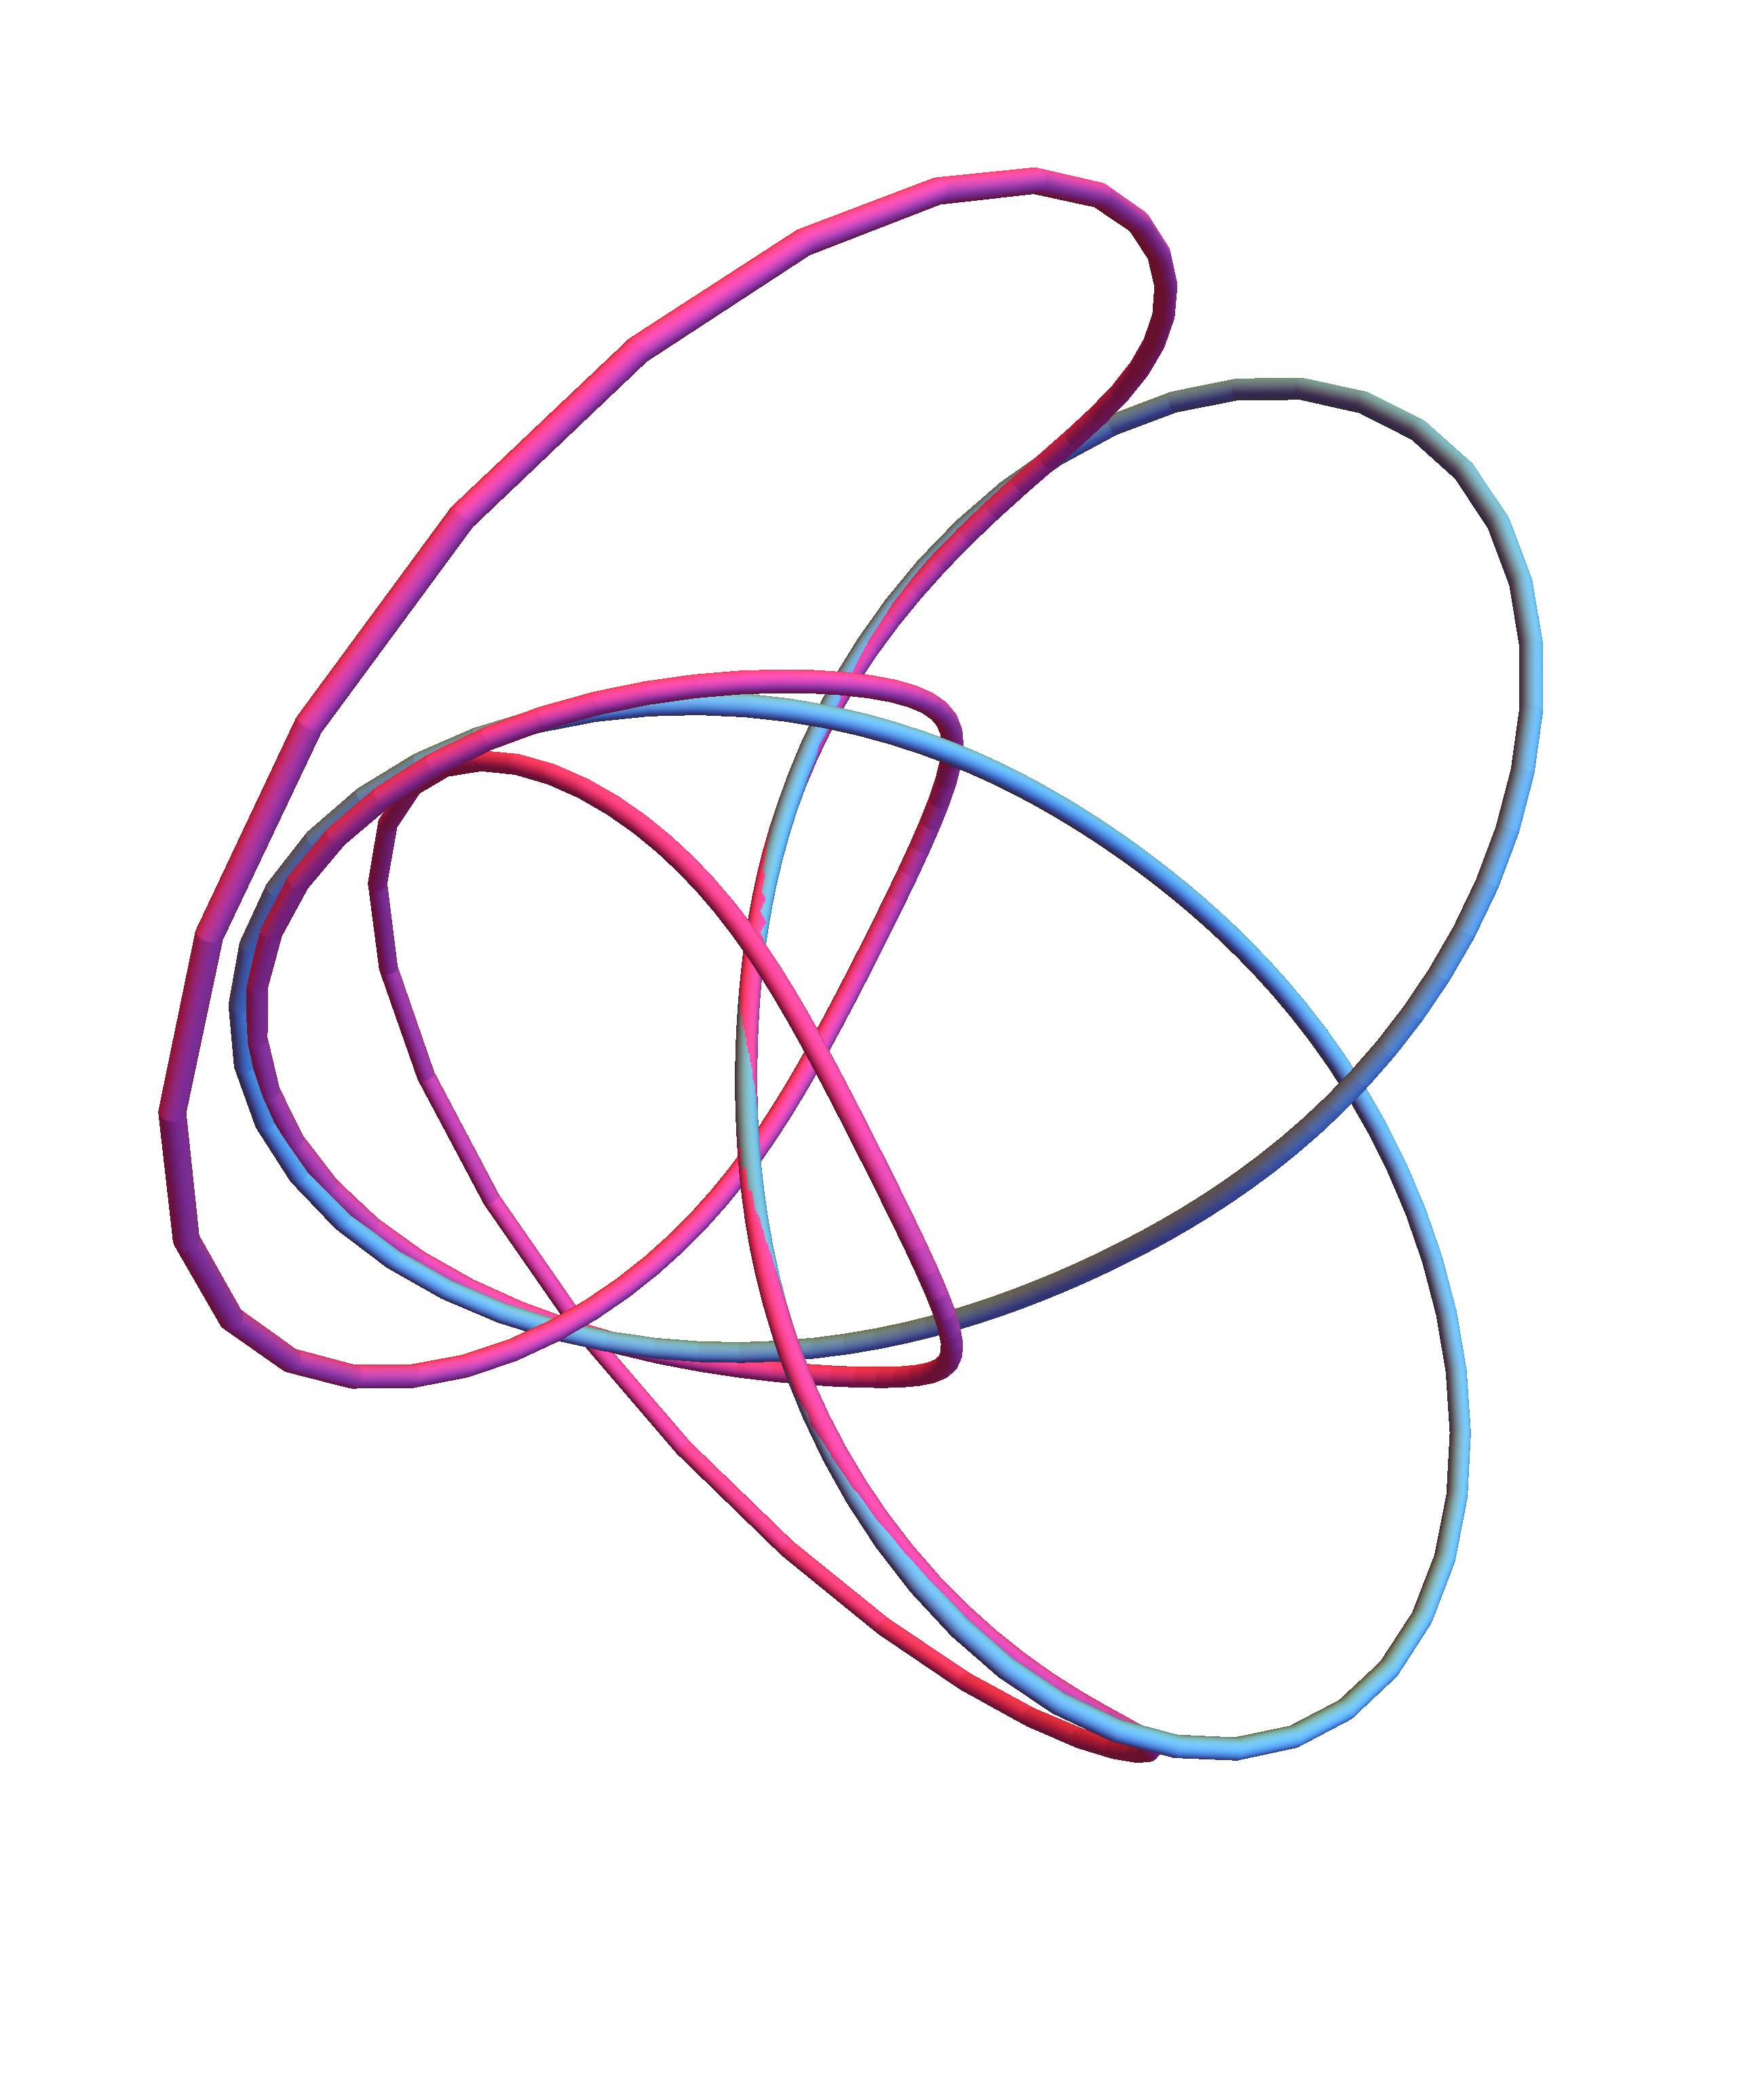
\includegraphics[width=0.4\linewidth]{figures/trefoil_link_pqqpqpppq.png}
  \caption{The modular trefoil link $k_A$ for $A = \protect\begin{psmallmatrix}32 & 25 \\ 23 & 18\protect\end{psmallmatrix}$.}
  \label{fig:trefoil_link_pqqpqpppq}
\end{figure}

\chapter{Finite subsets of the circle}\label{chap:finite_subsets}

\section{Topologizing $\exp_k X$}

We now arrive at our third homeomorphic space, the set of all nonempty subsets of $S^1$ with at most 3 points.
In general, we denote the set of all nonempty subsets with at most $k$ points of a space X as $\exp_k X$, and refer to it as a \defnphrase{finite subset space}.
Such a space can be given the topology induced by the quotient map
\begin{gather*}
  q : X^k \to \exp_k X \\
  q(x_1, x_2, \ldots, x_k) = \{x_1\} \cup \{x_2\} \cup \cdots \cup \{x_k\}
\end{gather*}
Alternatively, if the underlying space $X$ has metric structure, we can topologize $\exp_k X$ via an induced metric on subsets of $X$.
Let $d$ be a metric on $X$, and define the \defnphrase{$r$-inflation of $A \subseteq X$} as
\begin{equation*}
  A_r = \bigcup_{a \in A} \{ x \in X : d(a, x) < r \}
\end{equation*}
Then the \defnphrase{Hausdorff distance $d_H$} between two subsets $A$ and $B$ of $X$ is given by
\begin{equation*}
  d_H(A, B) = \inf \{ \varepsilon \geq 0 : A \subseteq B_\varepsilon, B \subseteq A_\varepsilon \}
\end{equation*}
Intuitively, the Hausdorff distance between two subsets is the smallest amount they must be ``inflated'' in order to contain each other.
The \defnphrase{Hausdorff metric topology} on $\exp_k X$ is the topology generated by the Hausdorff distance.

The Hausdorff metric topology provides a more instinctual notion of open sets in $\exp_k X$ than the above quotient topology, but results in literature concerning $\exp_k X$ often assume the quotient topology (which has the merit of not requiring additional metric structure on $X$).
For $X$ a metric space, however, it turns out that these two topologies are equivalent.
Since results in literature concerning $\exp_k X$ are sparse in general, we provide explicit proof of this fact.

\begin{prop}
  Let $(X, d)$ be a metric space.
  The Hausdorff metric topology $\mathcal{T}_H$ on $X$ is equivalent to the quotient topology $\mathcal{T}_q$ under the quotient map $q$.
\end{prop}

\begin{proof}
  To show that $\mathcal{T}_H \subseteq \mathcal{T}_q$, we will show that an arbitrary basis element for $\mathcal{T}_H$ is in $\mathcal{T}_q$.
  Since $\mathcal{T}_H$ is the metric topology generated by $d_H$, the set of all open balls in the metric $d_H$ is a basis for $\mathcal{T}_H$.
  Let $A = \{ a_1, a_2, \ldots, a_\ell \} \in \exp_k X$ and $r > 0$ a real number, so that $B(A, r)$ is an arbitrary open ball in $\mathcal{T}_H$.
  We claim that
  \begin{equation}\label{eq:subset_topologies_claim}
    q^{-1}(B(A,r)) = \bigcup_{\substack{x = (x_1, \ldots, x_k) \\ \in\ q^{-1}(B(A,r))}} B_d(x_1, r - r_x) \times \cdots \times B_d(x_k, r - r_x)
  \end{equation}
  where
  \begin{equation*}
    r_x = \max \{ d(x_i, a_j) : 1 \leq i \leq k,\ 1 \leq j \leq \ell \}
  \end{equation*}

  Let $y = (y_1, \ldots, y_k)$ be a point in the right-hand side of \eqref{eq:subset_topologies_claim}, so that $y \in \prod_i B_d(z_i,\ r - r_z)$ for some $z = (z_1, \ldots, z_k)$, and let $q(y)_r$ and $A_r$ be the $r$-inflation of $q(y)$ and $A$, respectively.
  Since each $y_i$ is in $B_d(z_i,\ r - r_z)$, we have that that $d(y_i, z_i) < r - r_z$.
  And for all $z_i$ there exists some $a_j \in A$ such that $d(z_i, a_j) < r_z$ (by construction of $r_z$).
  Then by the triangle inequality,
  \begin{equation*}
    d(y_i, a_j) \leq d(y_i, z_i) + d(z_i, a_j) < r - r_z + r_z = r
  \end{equation*}
  Thus $A \subseteq q(y)_r$.
  It can be shown similarly that $q(y) \subseteq A_r$ as well.
  It follows that $d_H(A, q(y)) < r$, hence $q(y) \in B(A,r)$ and $y \in q^{-1}(B(A,r))$. 
  
  Conversely, if $y \in q^{-1}(B(A,r))$, then it is clear that $y$ is in the union containing products of balls centered at the coordinates of $y$.
  So \eqref{eq:subset_topologies_claim} is verified.

  Then we have that $q^{-1}(B(A,r))$ is a union of finite products of open sets in $X$, and so $q^{-1}(B(A, r))$ is open in $X^k$.
  Thus we have that $\mathcal{T}_H$ is coarser than  $\mathcal{T}_q$.

  Now we will show that $\mathcal{T}_q \subseteq \mathcal{T}_H$ as well.
  Let $U \in \mathcal{U} \in \mathcal{T}_q$, and suppose that
  \begin{equation*}
    (x_1, \ldots, x_k) \in q^{-1}(U) \subseteq q^{-1}(\mathcal{U})
  \end{equation*}
  Since $q^{-1}(\mathcal{U})$ is open in $X^k$, we have that 
  \begin{equation*}
    q^{-1}(\mathcal{U}) = \bigcup_{j \in J} {V_j}_1 \times \cdots \times {V_j}_k
  \end{equation*}
  for some index set $J$, where each ${V_j}_i$ is open in $(X,d)$.
  Then $(x_1, \ldots, x_k) \in {V_j}_1 \times \cdots \times {V_j}_k$ for some $j \in J$.
  Since all ${V_j}_i$ are open in $(X,d)$, for each $x_i$ and some corresponding radius $r_i$ we can draw an open ball $B(x_i, r_i) \subseteq {V_j}_i$.
  So we have that
  \begin{equation*}
    (x_1, \ldots, x_k) \subseteq \prod_i B_d(x_i, r_i) \subseteq \prod_i {V_j}_i
  \end{equation*}
  Let $r = \min_i \{ r_i \}$.
  We claim that $B(U, r) \subseteq \mathcal{U}$: if it weren't, then there would exist some $W \in B(U, r)$ that is not in $\mathcal{U}$.
  But then there would exist some $w \in q^{-1}(W)$ such that $w \in \prod_i B_d(x_i, r_i)$ and $w \notin q^{-1}(\mathcal{U})$.
  This is a contradiction, since $\prod_i B_d(x_i, r_i) \subseteq q^{-1}(\mathcal{U})$.
  Thus we have that $B(U, r) \subseteq \mathcal{U}$.
  Since $U \in \mathcal{U}$ was arbitrary, this means that $\mathcal{U}$ is open in $(\exp_k X, \mathcal{T}_H)$, hence $\mathcal{T}_q \subseteq \mathcal{T}_H$.
\end{proof}

\section{From $\LS$ to $\exp_3 S^1$}\label{subsec:lattice_to_exp}

For our purposes, we will focus on a particular finite subset space, $\exp_3 S^1$.
In~\cite{mostovoy2004}, Mostovoy provides a homeomorphism $f : \LS \to \exp_3 S^1$, which we now describe.

The \defnphrase{Voronoi cell} $V(L)$ of a nondegenerate lattice $L$ is the cell in a Voronoi partition of $L$ containing $0$.
As a set,
\begin{equation*}
  V(L) = \{ z \in \C : |z| \leq |z - \omega| \text{ for all } \omega \in L \}
\end{equation*}
Sometimes this is also called the \defnphrase{Dirichlet region} or \defnphrase{Wigner-Seitz cell} of the lattice.
It is either a rectangle or a hexagon.

For nondegenerate $L \in \LS$, the homeomorphism $f$ is defined as follows.
Choose a vertex $v$ of $V(L)$.
If $L$ is rectangular, the minimum distance between $v$ and points of $L$ is obtained generically on two lattice points.
If $L$ is hexagonal, the minimum distance is obtained generically on three lattice points.
Consider the set of two or three lines connecting $v$ to the closest lattice points.
Translating $L$ so that $v$ is at the origin, we obtain two or three lines passing through the origin.
It is clear that these lines do not depend on the choice of vertex $v$ and are the same for any $L'$ homothetic to $L$.
Since lines passing through the origin are points in $\RP \cong S^1$, we have associated with each nondegenerate lattice $L$ a subset $f(L) \in \exp_3 S^1$.

Suppose instead that $L$ is a degenerate lattice, so that $L$ is contained within a line in $\RP$ passing through the origin.
We define $f$ for degenerate lattices by sending $L$ to this line.

For both degenerate and nondegenerate $L$, the verification of the continuity of $f$ is straightforward.
Several steps of the homeomorphism for nondegenerate $L$ are shown in Figure~\ref{fig:homeomorphism_to_subset}.

\begin{figure}[h]
  \centering
  \begin{subfigure}[t]{0.45\textwidth}
    \centering
    \includegraphics[width=\textwidth]{figures/subset_homeomorphism_step_1.pdf}
    \caption{A nondegenerate lattice in the plane.}
  \end{subfigure}
  \hfill
  \begin{subfigure}[t]{0.45\textwidth}
    \centering
    \includegraphics[width=0.8\textwidth]{figures/subset_homeomorphism_step_2.pdf}
    \caption{The Voronoi tessellation of the lattice, with a single hexagonal Voronoi cell selected.}
  \end{subfigure}
  \hfill
  \begin{subfigure}[t]{0.45\textwidth}
    \centering
    \includegraphics[width=0.8\textwidth]{figures/subset_homeomorphism_step_3.pdf}
    \caption{The three closest lattice points to any vertex the cell define three lines in $\RP$.}
  \end{subfigure}
  \hfill
  \begin{subfigure}[t]{0.45\textwidth}
    \centering
    \includegraphics[width=0.7\textwidth]{figures/subset_homeomorphism_step_4.pdf}
    \caption{The three lines in $\RP \cong S^1$ define three points on the circle.}
  \end{subfigure}
  \caption{Various stages of the homeomorphism $\LS \to \exp_3 S^1$.}
  \label{fig:homeomorphism_to_subset}
\end{figure}

\section{Visualizing the generators of $B_3$ in $\exptwothree S^1$}

Observe that the homeomorphism $f : \LS = \LS_0 \cup \LS_1 \to \exp_3 S^1$ sends the subspace $\LS_0 $ to $\exp_1 S^3$ and the subspace $\LS_1$ to the 2 and 3 point elements of $\exp_3 S^1$.
We will denote this subspace of 2 and 3 point elements as $\exptwothree S^1$.

In Chapter~\ref{sec:three_sphere}, we showed that $\pi_1(S^3 \wo K)$ was the braid group $B_3$, and that the trefoil knot $K$ corresponded to degenerate lattices under the homeomorphism $\LS \to S^3$.
Thus we have that
\begin{equation*}
  \pi_1(\exptwothree S^1) = \pi_1(\LS_1) = \pi_1(S^3 \wo K) = B_3
\end{equation*}
We now wish to describe the generators $\sigma_1$ and $\sigma_2$ of $B_3$ visually in $\exptwothree S^1$.
That is, we wish to find representatives of the path classes $\sigma_1$ and $\sigma_2$.

In computing the fundamental group of $S^3 \wo K$, we understood the path classes generating a group $\ang{x, y : x^2 = y^3} \cong B_3$.
The generator $x$ was a path through the axis of a particular solid torus in $S_3$, while $y$ was a large loop linking the hole of the torus.
Explicitly, we can parametrize these paths by $(e^{i \theta}, 0)$ and $(0, e^{i \theta})$ where $\theta \in [0, 2 \pi]$.
Pushing these paths via homeomorphisms $S^3 \to \LS \to \exp_3 S^1$ yields two paths in $\exp_3 S^1$: a ``half twist'' and ``third twist'' of two or three equally spaced points, respectively.

\begin{figure}[t]
  \centering
  \begin{subfigure}[c]{0.32\textwidth}
    \centering
    \includegraphics[width=0.9\textwidth]{figures/s3_wo_k_gens.png}
  \end{subfigure}
  \hfill
  \begin{subfigure}[c]{0.32\textwidth}
    \centering
    \includegraphics[width=0.9\textwidth]{figures/antipodal_subset_path_1.pdf}
  \end{subfigure}
  \hfill
  \begin{subfigure}[c]{0.32\textwidth}
    \centering
    \includegraphics[width=0.9\textwidth]{figures/antipodal_subset_path_2.pdf}
  \end{subfigure}
  \caption{The knot complement space $S^3 \wo K$ has a fundamental group generated by two loops $x$ and $y$, shown in the left figure as the orange and pink loops, respectively (the pink strand is a loop according to the decomposition of $S^3$ as $S^1 \times D^2 \cup D^2 \times S^1$). The trefoil knot $K$ is shown in blue. On the right, we visualize these generators as string cheese diagrams by pushing the generators through the sequence of homeomorphisms from $S^3$ to $\exp_3 S^1$, where they present as a half or third twist of equally space points.}
  \label{fig:antipodal_point_paths}
\end{figure}


We visualize these paths in Figure~\ref{fig:antipodal_point_paths} using a style of planar diagram we call a \defnphrase{string cheese diagram}.
In a string cheese diagram, the horizontal axis is scaled from 0 to $2\pi$ and opposite edges of the diagram are identified.
Each horizontal slice of the diagram contains two or three points, and thus represents a point in $\exptwothree S^1$.
The vertical axis is scaled from the beginning to the end of a loop in $\exptwothree S^1$, which will start and end on the same two or three points (i.e. the same single element of $\exptwothree S^1$).
The aesthetic of a continuous path in these diagrams is striking; we see that a path may collapse from three points to two points, or split from two points to three points \` a la ``string cheese''.

A string cheese diagram is most useful for understanding compositions of paths that share a common basepoint, like the elements in a fundamental group.
The composition of paths in $\pi_1(\exptwothree S^1)$ is computed by simply stacking multiple string cheese diagrams one after another.
In this sense, the string cheese diagrams are in the same spirit as other visual calculi, such as the diagrammatic computations found of the braid group, of the Temporly-Lieb algebra, or in Pawel Sobocinski's ``Graphical Linear Algebra''~\cite{graphicallinearalgebra}.
An example of path composition in $\exptwothree S^1$ will be shown shortly.

\begin{figure}[h]
  \centering
  \begin{subfigure}[t]{0.23\textwidth}
    \centering
    \includegraphics[width=\textwidth]{figures/braid_gen_x.pdf}
  \end{subfigure}
  \hspace{5mm}
  \begin{subfigure}[t]{0.23\textwidth}
    \centering
    \includegraphics[width=\textwidth]{figures/braid_gen_y.pdf}
  \end{subfigure}
  \caption{The representatives of the generators $x$ and $y$ of $\exptwothree S^1$, modified to share a common basepoint.}
  \label{fig:common_basepoint_generators}
\end{figure}

To employ these diagrams in our analysis of the generators of $\pi_1(\exptwothree S^1)$, we first modify the half and third twist generators from Figure~\ref{fig:antipodal_point_paths} to share a common basepoint.
These modified loops are shown in Figure~\ref{fig:common_basepoint_generators}.
Then, using the inverse of the isomorphism $\pi_1(S^3 \wo K) \to B_3$ defined in \eqref{eq:iso_pi1_b3}, we have that
\begin{align*}
  \sigma_1 &= y^{-1} x \\
  \sigma_2 &= x^{-1} y^2.
\end{align*}
The compositions $y^{-1} x$ and $x^{-1} y^2$ are shown in Figure~\ref{fig:braid_gen_equals}, which yield diagrams of the braid group generators $\sigma_1$ and $\sigma_2$ that we seek.
The diagrams for the inverses of $\sigma_1$ are $\sigma_2$ are shown in Figure~\ref{fig:braid_gen_invs_exp}.

\begin{figure}[h]
  \centering
  \begin{subfigure}[c]{0.47\textwidth}
    \centering
    \includegraphics[width=\linewidth]{figures/braid_gen_y_inv_x_equals.pdf}
    \caption{$\sigma_1 = y^{-1} x$}
  \end{subfigure}
  \hfill
  \begin{subfigure}[c]{0.47\textwidth}
    \centering
    \includegraphics[width=\linewidth]{figures/braid_gen_x_inv_y_y_equals.pdf}
    \caption{$\sigma_2 = x^{-1}y^2$}
  \end{subfigure}
  \caption{Computing the braid group generators in $\exptwothree$ via composing string cheese diagrams.}
  \label{fig:braid_gen_equals}
\end{figure}

\begin{figure}[h]
  \centering
  \begin{subfigure}[t]{0.23\textwidth}
    \centering
    \includegraphics[width=\textwidth]{figures/braid_gen_a_inv.pdf}
    \caption{$\sigma_1^{-1}$}
  \end{subfigure}
  \hspace{5mm}
  \begin{subfigure}[t]{0.23\textwidth}
    \centering
    \includegraphics[width=\textwidth]{figures/braid_gen_b_inv.pdf}
    \caption{$\sigma_2^{-1}$}
  \end{subfigure}
  \caption{Representatives for the inverse generators $\sigma_1^{-1}$ and $\sigma_2^{-1}$ of $\pi_1(\exptwothree S^1)$.}
  \label{fig:braid_gen_invs_exp}
\end{figure}

The braid group $B_3$ has a single relation, which we saw visualized Figure~\ref{fig:visual_braid_group}.
We can now visualize this same relation in $\exptwothree S^1$ using via string cheese diagrams.
The relation is shown in Figure~\ref{fig:braid_relation_exp}.

\begin{figure}[h]
  \centering
  \includegraphics[width=0.8\linewidth]{figures/braid_relation_exp.pdf}
  \caption{The braid relation $\sigma_1 \sigma_2 \sigma_1 = \sigma_2 \sigma_1 \sigma_2$ in $\pi_1(\exptwothree S^1)$.}
  \label{fig:braid_relation_exp}
\end{figure}

\section{Diagrammatic decompositions of hyperbolic subset loops}

Previously we saw that the periodic orbits of a dynamical system in $\LS_1$ were in bijection with conjugacy classes of hyperbolic elements in $\SLZ$, and that each conjugacy class determined a modular knot in $S^3 \wo K$.
We can also examine these periodic orbits as loops in $\exptwothree S^1$ via the homeomorphism $\LS \to \exp_3 S^1$.
Several such loops are shown in Figure~\ref{fig:subset_loop_examples}; it may be interesting to compare them to the knots in $S^3 \wo K$ produced by the same hyperbolic matrices in Figure~\ref{fig:trefoil_links}.
When viewed in $\exptwothree S^1$, we call these periodic orbits \defnphrase{hyperbolic subset loops}.

\begin{figure}[h]
  \centering
  \begin{subfigure}[t]{0.31\textwidth}
    \centering
    \includegraphics[width=\textwidth]{figures/subset_loop_qp_1_1_1_2.pdf}
    \caption*{$A = \begin{pmatrix}1 & 1 \\ 1 & 2\end{pmatrix}$}
  \end{subfigure}
  \hfill
  \begin{subfigure}[t]{0.31\textwidth}
    \centering
    \includegraphics[width=\textwidth]{figures/subset_loop_pqpq_5_3_3_2.pdf}
    \caption*{$A = \begin{pmatrix}5 & 3 \\ 3 & 2\end{pmatrix}$}
  \end{subfigure}
  \hfill
  \begin{subfigure}[t]{0.31\textwidth}
    \centering
    \includegraphics[width=\textwidth]{figures/subset_loop_pqqq_4_1_3_1.pdf}
    \caption*{$A = \begin{pmatrix}4 & 1 \\ 3 & 1\end{pmatrix}$}
  \end{subfigure}
  \caption{Conjugacy classes of hyperbolic $A \in \SLZ$ are in bijection with period orbits of a dynamical system in $\LS$. These periodic orbits can be examined as loops in $\exptwothree S^1 \approx \LS_1$. Here, several loops are shown in $\exptwothree S^1$ for various values of $A \in \SLZ$.}
  \label{fig:subset_loop_examples}
\end{figure}

The path class of each of these hyperbolic subset loops is an element of the group $\pi_1(\exptwothree S^1)$, which is isomorphic to the braid group $B_3$.
In particular, each loop is a braid word in $\sigma_1$ and $\sigma_2$, the generators of $B_3$.
In the previous section, we found visual representatives for $\sigma_1$ and $\sigma_2$.
Given a diagram of a hyperbolic subset loop, can we decompose it into a word in $\sigma_1$ and $\sigma_2$?

We demonstrate that such a decomposition is possible with the following steps:
\begin{enumerate}[1.]
  \item If necessary, first shift the hyperbolic subset loop diagram so that the top and bottom edges correspond to a 3-pointed element of $\exptwothree S^1$.
  Since the diagram represents a loop, we are free to choose which point in the loop is the starting and ending point.

  \item Perform a series of homotopy-class preserving deformations to simplify the diagram.
  These deformations must be homotopies. In particular, at no time can the deformed loop diagram have a 1-point element. 

  \item Identify a sequence of $\sigma_1$ and $\sigma_2$ diagrams that can be homotopy-transformed back to the diagram in the previous step.
\end{enumerate}

This process is shown for two separate hyperbolic subset loop diagrams in Figure~\ref{fig:subset_loop_decompositions_1} and Figure~\ref{fig:subset_loop_decompositions_2}.
The results for decomposing several more diagrams are presented in Figure~\ref{fig:subset_loop_decompositions_table}.

We know that every modular trefoil knot has a corresponding representation as an element of the braid group because we computed $\pi_1(S^3 \wo K)$ directly.
However, this computation was achieved via the sprawling and opaque machinery of the Seifart Van-Kampen theorem, and provides little insight into how we ought to intuit modular trefoil knots as braids.
Decomposing string cheese diagrams provides us with our concrete examples of braids and their corresponding modular trefoil links.
What can we now say about modular trefoil links as braids?

The braid word $\beta_A$ for a modular trefoil link $k_A$ mimics the $PQ$ decomposition of $A$ closely.
For example, $A = PQQ$ is $\sigma_2 \sigma_2 \sigma_1^{-1}$ as a braid, while $A  = PQQQ$ is $\sigma_2 \sigma_2 \sigma_2 \sigma_1^{-1}$.
Notice that every character in the $PQ$ word has exactly one matching character in the braid word.
These matchings vary throughout the different example braids---sometimes $Q$ corresponds to $\sigma_1$ in a braid word, but other times it corresponds to $\sigma_2$---but for each individual $(k_A, \beta_A)$ pairing there is some one-to-one correspondence between characters $P$ and $Q$ in $A$ and characters $\sigma_i^{\pm 1}$ in $\beta_A$.

There may still exist a map between $\SLZ$ and $B_3$ that utilizes $PQ$ decompositions of elements in $\SLZ$.
Every braid $\beta_A$ for a modular trefoil link $k_A$ was obtained via a decomposition of the string cheese diagram for $k_A$. 
Did we make subtle and arbitrary choices in the decomposition process that affects whether $P$ maps to $\sigma_2^{-1}$ or $\sigma_1^{-1}$, and whether $Q$ maps to $\sigma_1$ or $\sigma_2$?
Or does the sign of the braid group generators reflect the orientation of the modular trefoil link?
Or yet still, are some of these braid words equivalent? These questions remain open.

\begin{figure}[p]
  \centering
  \begin{subfigure}[t]{0.24\linewidth}
    \centering
    \includegraphics[height=5cm]{figures/subset_loop_ppqq.pdf}
    \caption{}
  \end{subfigure}
  \hfill
  \begin{subfigure}[t]{0.24\linewidth}
    \centering
    \includegraphics[height=5cm]{figures/subset_loop_ppqq_shifted.pdf}
    \caption{}
  \end{subfigure}
  \hfill
  \begin{subfigure}[t]{0.24\linewidth}
    \centering
    \includegraphics[height=5cm]{figures/subset_loop_ppqq_normalized.pdf}
    \caption{}
  \end{subfigure}
  \hfill
  \begin{subfigure}[t]{0.24\linewidth}
    \centering
    \includegraphics[height=5cm]{figures/subset_loop_ppqq_decomposed.pdf}
    \caption{}
  \end{subfigure}
  \caption{Decomposing the hyperbolic subset loop diagram for $A = 
  \protect\begin{psmallmatrix}5 & 2 \\ 2 & 1\protect\end{psmallmatrix}$ into braid group generators. The diagram in (a) depicts the unmodified periodic orbit in $\LS$ corresponding to $A$ after it has been pushed $\LS \to \exptwothree S^1$ via a homeomorphism. In (b), the diagram has been shifted so that it begins and ends on a 3-point element of $\exptwothree S^1$. In (c), the diagram has been continuously deformed to represent a path within the same homotopy class. In (d), the deformed diagram has been decomposed into a sequence of $\sigma_1$ and $\sigma_2$ diagrams, whose composition is still within the same homotopy class. The sequence is the braid $\sigma_2^{-1} \sigma_2^{-1} \sigma_1 \sigma _1$.} 
  \label{fig:subset_loop_decompositions_1}
\end{figure}

\begin{figure}[p]
  \centering
  \begin{subfigure}[t]{0.24\linewidth}
    \centering
    \includegraphics[height=5cm]{figures/subset_loop_pqq.pdf}
  \end{subfigure}
  \hfill
  \begin{subfigure}[t]{0.24\linewidth}
    \centering
    \includegraphics[height=5cm]{figures/subset_loop_pqq_shifted.pdf}
  \end{subfigure}
  \hfill
  \begin{subfigure}[t]{0.24\linewidth}
    \centering
    \includegraphics[height=5cm]{figures/subset_loop_pqq_normalized.pdf}
  \end{subfigure}
  \hfill
  \begin{subfigure}[t]{0.24\linewidth}
    \centering
    \includegraphics[height=5cm]{figures/subset_loop_pqq_decomposed.pdf}
  \end{subfigure}
  \caption{Decomposing the hyperbolic subset loop diagram for $A = \protect\begin{psmallmatrix}3 & 1 \\ 2 & 1\protect\end{psmallmatrix}$ into braid group generators, with the same process described in Figure~\ref{fig:subset_loop_decompositions_1}.}
  \label{fig:subset_loop_decompositions_2}
\end{figure}

\begin{figure}[p]
  \centering
  \begin{tabular}{r l}
   hyperbolic matrix & hyperbolic subset loop decomposition \\
   \toprule
   $PQ = \begin{pmatrix}2 & 1 \\ 1 & 1\end{pmatrix}$ & $\sigma_2 \sigma_1^{-1}$ \\[1em]
   $PQQ = \begin{pmatrix}3 & 1 \\ 2 & 1\end{pmatrix}$ & $\sigma_2 \sigma_2 \sigma_1^{-1}$ \\[1em]
   $PQQQ = \begin{pmatrix}4 & 1 \\ 3 & 1\end{pmatrix}$ & $\sigma_2 \sigma_2 \sigma_2 \sigma_1^{-1}$ \\[1em]
   $PQQQQ = \begin{pmatrix}5 & 1 \\ 4 & 1\end{pmatrix}$ & $\sigma_2 \sigma_2 \sigma_2 \sigma_2 \sigma_1^{-1}$ \\[1em]
   $PPPQ = \begin{pmatrix}4 & 3 \\ 1 & 1\end{pmatrix}$ & $\sigma_2^{-1} \sigma_1 \sigma_2^{-1} \sigma_2^{-1}$ \\[1em]
   $PPPQQ = \begin{pmatrix}7 & 3 \\ 2 & 1\end{pmatrix}$ & $\sigma_2^{-1} \sigma_2^{-1} \sigma_1 \sigma_1 \sigma_2^{-1}$ \\[1em]
   $PPPPQ = \begin{pmatrix}5 & 4 \\ 1 & 1\end{pmatrix}$ & $\sigma_2^{-1} \sigma_2^{-1} \sigma_2^{-1} \sigma_1 \sigma_2^{-1}$ \\[1em]
   $PPQ = \begin{pmatrix}3 & 2 \\ 1 & 1\end{pmatrix}$ & $\sigma_1 \sigma_2^{-1} \sigma_2^{-1}$ \\[1em]
   $PPQQ = \begin{pmatrix}5 & 2 \\ 2 & 1\end{pmatrix}$ & $\sigma_2^{-1} \sigma_2^{-1} \sigma_1 \sigma_1$ \\[1em]
   $PPQQQ = \begin{pmatrix}7 & 2 \\ 3 & 1\end{pmatrix}$ & $\sigma_2^{-1} \sigma_2^{-1} \sigma_1 \sigma_1 \sigma_1$ \\[1em]
   $PQPQ = \begin{pmatrix}5 & 3 \\ 3 & 2\end{pmatrix}$ & $\sigma_2 \sigma_1^{-1} \sigma_2 \sigma_1^{-1}$ \\[1em]
   $PQPQP = \begin{pmatrix}5 & 8 \\ 3 & 5\end{pmatrix}$ & $\sigma_2^{-1} \sigma_2^{-1} \sigma_1 \sigma_2^{-1} \sigma_1$
  \end{tabular}
  \caption{Decompositions of hyperbolic subset loops corresponding to twelve hyperbolic matrices. Each matrix is in a unique conjugacy class, and thus produces a unique hyperbolic subset loop.}
  \label{fig:subset_loop_decompositions_table}
\end{figure}

\section{The linking number of finite subset loops}

Pushing modular knots into $\exptwothree S^1$ enables the decomposition of their path classes as braid words.
More generally, it also provides a rich variety of modular knots examples that can be studied in a new setting.
Can we recover any of the known results about modular knots from the perspective of $\exp_{2,3} S^1$?
We conclude this thesis with a conjecture concerning the linking number of hyperbolic subset loops.

Every point along a hyperbolic subset loop is a two- or three-pointed subset of $S^1$.
In a string cheese diagram, the two-pointed subsets of the loop are easily identified and appear only a finite number of times.
At each of these two-pointed subsets, an incoming fork and outgoing fork are visible.
Furthermore, the incoming strand to the outgoing fork has an orientation; it is either approaching from the left or right side of the diagram (see Figure~\ref{fig:subset_loop_forks}). 
If the incoming strand to the outgoing fork approaches from the left in a string cheese diagram, we call the outgoing fork a \defnphrase{left fork}.
Otherwise, the outgoing fork is a \defnphrase{right fork}.

\begin{figure}[h]
  \centering
  \begin{subfigure}[t]{0.31\textwidth}
    \centering
    \includegraphics[width=\textwidth]{figures/subset_loop_forks_ppqq.pdf}
    \caption*{$A = PPQQ$}
  \end{subfigure}
  \hspace{5mm}
  \begin{subfigure}[t]{0.31\textwidth}
    \centering
    \includegraphics[width=\textwidth]{figures/subset_loop_forks_pqqq.pdf}
    \caption*{$A = PQQQ$}
  \end{subfigure}
  \caption{Two string cheese diagrams corresponding to the modular knot $k_A$ where $A \in \SLZ$. The outgoing forks in each diagram are highlighted. If the incoming strand to an outgoing fork approaches from the left, we call the fork a \defnphrase{left fork} (highlighted in blue). Otherwise, it is a \defnphrase{right fork} (highlighted in purple). We conjecture that the linking number of a modular knot $k_A$ is the number of left forks minus the number of right forks in a string cheese diagram for $k_A$.}
  \label{fig:subset_loop_forks}
\end{figure}

\begin{conj}
  Let $m$ and $n$ be the number of left and right forks, respectively, in a string cheese diagram of a modular knot $k_A$.
  Then the linking number of $k_A$ is $m - n$.
\end{conj}

This conjecture is motivated empirically by a large set of string cheese diagrams for which the statement holds true.
Recall that every conjugacy class of a hyperbolic element of $\PSLZ$ has a $PQ$-decomposition (Corollary~\ref{prop:pq_decomposition}), and that the trace of a matrix in $\PSLZ$ is an invariant of its conjugacy class (Lemma~\ref{lemma:tr_is_conj_invariant}).
It's readily verified that multiplication by $P$ or $Q$ increases the trace of a hyperbolic $PQ$ word.
Thus to enumerate the conjugacy classes of hyperbolic elements of $\PSLZ$, we can enumerate words in $P$ and $Q$ (taking care to omit words containing cycles and starting with $PQ$).
In Appendix~\ref{sec:coding_ls_to_exp}, we supply a computer program that outputs a string cheese diagram given a $PQ$ word.
We produced 28 string cheese diagrams for $PQ$ words corresponding to 28 unique conjugacy classes of elements in $\PSLZ$ and verified the conjecture in each case  by applying Theorem~\ref{thm:ghys} to the $PQ$ words and by visually inspecting the diagrams.

\newpage
\appendix

\chapter{Computational exploration of homeomorphisms}

Steve Jobs believed that a computer is a ``bicycle for the mind''\cite{krainin1990}.
We can't tell computers what to think, but we can employ them to make our own thinking more efficient.
This observation is now so widely realized as to be banal---in every other field besides mathematics, at least.
Mathematics, however, remains less affected by developments in computing.

By its nature, math seeks knowledge about objects that defy computational interpretation.
It seeks to describe properties of all real numbers and not just those that we can store in a finite bank of computer memory.
While some progress has been made in articulating mathematical knowledge as computer programs, computers will continue to be of secondary importance in mathematics for the foreseeable future.
We can, however, use computers to generate intuition and to suggest what purely analytical questions we might ask next.

The results in this document were explored and understood via computer programming.
What follows now is a ``literate programming'' description of the relevant Mathematica programs~\cite{knuth1992}.
Some knowledge of Mathematica programming is assumed.
These programs and other digital supplements to this thesis will be made available on the Reed Electronic Thesis Archive\footnote{\url{https://rdc.reed.edu/c/etheses/home/}} as well as on GitHub\footnote{\url{https://github.com/chnn}}.

\newpage

\section{Visualizing a dynamic system in the space of lattices}

A lattice is uniquely defined by its generators, a pair of complex numbers.
This suggests we can encode lattices programmatically in a simple manner as \texttt{\{w1, w2\}}, where \texttt{w1} and \texttt{w2} are the complex generators. 

In Section~\ref{subsec:lattice_flow}, we considered a lattice produced by a $2 \times 2$ matrix acting point-wise upon the standard square lattice, $\Z \oplus \Z$.
Given a lattice, we can find this corresponding matrix:
\begin{minted}[breaklines, fontsize=\small]{Mathematica}
latticeToMtx[m_] := m // ReIm // Transpose;
\end{minted}
We can also convert back to a lattice from the matrix form:
\begin{minted}[breaklines, fontsize=\small]{Mathematica}
mtxToLattice[m_] := (Complex @@ #)& /@ Transpose[m];
\end{minted}
These are just simple accessors to get data representing a lattice into a convenient shape.
We can now describe the dynamical system of Proposition~\ref{prop:hyperbolic_defines_flow}.
Suppose that $A \in \SLZ$, and let $P$ such that $PAP^{-1} = \delta_t$, where $\delta_t$ is defined as in \eqref{eq:delta_t}.
Then $P$ is a matrix whose columns are the eigenvectors of $A$, thus we can compute the lattice corresponding to $P$ with the function 
\begin{minted}[breaklines, fontsize=\small]{Mathematica}
latticeForModularMtx[a_] := a // Eigenvectors // N // Transpose // Inverse // mtxToLattice;
\end{minted}
where \mintinline{Mathematica}|a| is the Mathematica representation of $A$.
Remember that we obtain the dynamical system of interest by acting upon $P$ via $\delta_t$ for continuously increasing $t$.

To observe a periodic orbit in this system, we need a programmatic method for obtaining the orbit time.
That is, we wish to find a minimal $T > 0$ such that $\delta_T P = P$.
We know that $PAP^{-1} = \delta_T$ is a diagonal matrix with diagonal entries being eigenvalues of $A$.
And since
\begin{equation*}
  \delta_T = \begin{pmatrix}
    \exp(T) & 0 \\
    0 & \exp(-T)
  \end{pmatrix}
\end{equation*}
these eigenvalues are in fact $\exp(T)$ and $\exp(-T)$.
Thus we can take the logarithm of the absolute value of either eigenvalue to obtain the orbit time $T$.
In Mathematica, we do so with the following function:
\begin{minted}[breaklines, fontsize=\small]{Mathematica}
orbitTimeForModularMtx[m_] := m // Eigenvalues // N // First // Abs // Log;
\end{minted}

With the appropriate matrix $P$ corresponding to some $A \in \SLZ$ and the orbit time readily available, we can now encode the path of a periodic orbit in the space of lattices.
First, we define a quick utility function for $\delta_t$:
\begin{minted}[breaklines, fontsize=\small]{Mathematica}
deltaT[t_] := {{E^t, 0}, {0, E^-t}} // N;
\end{minted}
Then an ordered list of points along the periodic orbit can be computed as follows:
\begin{minted}[breaklines, fontsize=\small]{Mathematica}
assocLatticeLoop[mtx_, res_: 100] := Module[{p, t},
   p = latticeToMtx[latticeForModularMtx[mtx]];
   t = orbitTimeForModularMtx[mtx];
   Table[mtxToLattice[deltaT[u].p], {u, 0, t, t / res}]
   ];
\end{minted}
There are, of course, infinitely many points along the path of the periodic orbit, of which we can only compute a finite number.
We parameterize the amount of points along the path to compute with the resolution parameter \mintinline{Mathematica}|res|.

How can we visualize these periodic orbits?
Each point in the periodic orbit is a lattice, and we can readily visualize a subset of each lattice in the plane.
Thus a natural visualization choice for the periodic orbits is an animation, with each frame being a depiction of a lattice in the plane.
The following function produces a subset of the points in a lattice:
\begin{minted}[breaklines, fontsize=\small]{Mathematica}
latticePoints[{w1_, w2_}, size_: 1] := ReIm /@ Flatten[ Table[m w1 + n w2, {m, Range[-size, size]}, {n, Range[-size, size]}]];
\end{minted}
Then the desired animation is produced by:
\begin{minted}[breaklines, fontsize=\small]{Mathematica}
visualizeLatticeLoop[ls_] := ListAnimate[ListPlot[latticePoints[#, 100], PlotRange -> {{-2, 2}, {-2, 2}}]& /@ assocLatticeLoop[ls]]
\end{minted}
It's difficult to print a movie onto a piece of paper, so we show a static adaptation of this animation in Figure~\ref{fig:periodic_orbits_lattice}.

\section{Coding the homeomorphism from $\LS \to S^3$}

We now have a program capable of realizing the periodic orbits of a dynamical system in the space of lattices.
In the homeomorphic space $S^3$, these periodic orbits appear as links with the trefoil.
In this section, we will code the homeomorphism from $\LS$ to $S^3$ described in Section~\ref{sec:lattice_to_s3}, and use it to visualize links with the trefoil.

The homeomorphism $\LS \to S^3$ sends a lattice $L$ to a rescaled version of the complex tuple $(G_4(L),\, G_6(L))$, where
\begin{equation*}
  G_k(L) = \sum_{\omega \in L,\ \omega \neq 0} \omega^{-k}
\end{equation*}
A nontrivial lattice $L$ contains infinitely many points $\omega$, presenting a potential challenge in computing $G_k(L)$.
The series for $G_4(L)$ and $G_6(L)$ do converge however, and for nondegenerate lattices we can compute the tuple $(G_4(L),\, G_6(L))$ using Mathematica's \mintinline{Mathematica}|WeierstrassInvariants| function.
The \mintinline{Mathematica}|WeierstrassInvariants| function (more commonly used in cryptographic applications) returns two special constants $g_2$ and $g_3$ associated with a lattice.
These are related to $G_4(L)$ and $G_6(L)$ by $g_2(L) = G_4(L) / 60$ and $g_3(L) = G_6(L) / 140$.
Thus the Mathematica function
\begin{minted}[breaklines, fontsize=\small]{Mathematica}
nondegenGTuple[{w1_, w2_}] := N[WeierstrassInvariants[{w1/2, w2/2}]] * {1/60, 1/140} // Chop;
\end{minted}
returns our desired point $(G_4(L),\, G_6(L))$ for nondegenerate $L \in \LS$.
What about degenerate lattices?
In this case, the series $G_k(L)$ converge fast enough that we can leverage a straightforward numerical approach.
We start computing the infinite series from the origin outwards, and let Mathematica determine when we have reached reasonable numeric accuracy:
\begin{minted}[breaklines, fontsize=\small]{Mathematica}
degenEisensteinSeries[c_, k_] := N[Sum[(n c)^-k+ (-n c)^-k, {n, \[Infinity]}]];

degenGTuple[c_] := {degenEisensteinSeries[c, 4], degenEisensteinSeries[c, 6]};
\end{minted}
Now, the next step in the homeomorphism is to rescale the tuple $(G_4(L), G_6(L))$ so that it lies in $S^3 = \{(u,\, v) \in \C : |u|^2 + |v|^2 = 1\}$.
Recall that for any real number $t > 0$ and lattice $L$, we have that
\begin{equation*}
  G_4(tL) = t^{-4}G_4(L)
\end{equation*}
and
\begin{equation*}
  G_6(tL) = t^{-6} G_6(L)
\end{equation*}
Thus we solve for the appropriate scaling factor $t$ so that $(G_4(tL), G_6(tL))$ is in $S^3$:
\begin{minted}[breaklines, fontsize=\small]{Mathematica}
gTupleScaleFactor[{g4_, g6_}] := t /.Solve[Norm[t^-4 g4]^2 + Norm[t^-6 g6]^2 == 1 && t  \[Element] Reals && t > 0, t][[1]] // Quiet;
\end{minted}

We're almost ready to code the complete homeomorphism $\LS \to S^3$.
The last gadget we need is a utility function to check if a lattice is degenerate, so that we know when to branch into our seperate \mintinline{Mathematica}|nondegenGTuple| and \mintinline{Mathematica}|degenGTuple| functions.
A degenerate lattice either has a zero generator, or has rank one in matrix form.
\begin{minted}[breaklines, fontsize=\small]{Mathematica}
isDegen[{w1_, w2_}] := w1 == 0 || w2 == 0 || MatrixRank[{ReIm[w1], ReIm[w2]}] == 1;
\end{minted}
Now we can wire up our previously defined functions to form the complete homeomorphism.
\begin{minted}[breaklines, fontsize=\small]{Mathematica}
latticeToS3[l_] := Module[{gTuple, t},
  gTuple = If[isDegen[l],degenGTuple[degenGenerator[l]], nondegenGTuple[l]]; 
  t = gTupleScaleFactor[gTuple];
  {t^-4, t^-6} * gTuple
];
\end{minted}
As discussed in Section~\ref{sec:lattice_to_s3}, all degenerate lattices in $\LS$ present as a trefoil when viewed in $S^3$.
We can see this via our coded homeomorphism as follows.
First, we define a function that will help us parameterize a path through all degenerate lattices.
\begin{minted}[breaklines, fontsize=\small]{Mathematica}
  degenLatticeForAngle[rad_] := N[{Complex @@ radToR2[rad], Complex @@ radToR2[rad]}];
\end{minted}
Since $S^3$ lies within four-dimensional space, we also need to sterographically project points of $S^3$ into $\R^3$ before we can visualize them.
\begin{minted}[breaklines, fontsize=\small]{Mathematica}
  projS3ToR3[{z1_, z2_}] := {Re[z1]/(1 - Im[z2]), Im[z1]/(1 - Im[z2]), Re[z2]/(1 - Im[z2])};
\end{minted}
Now we can generate the points of the trefoil knot:
\begin{minted}[breaklines, fontsize=\small]{Mathematica}
  trefoilPoints = Table[degenLatticeForAngle[r] // latticeToS3 // projS3ToR3, {r, 0, Pi, 0.02}];
\end{minted}
And then visualize the trefoil, as shown in Figure~\ref{fig:trefoil}:
\begin{minted}[breaklines, fontsize=\small]{Mathematica}
  trefoilPlot = Graphics3D[{Thick, Blue, Tube[trefoilPoints]}, Boxed -> False]
\end{minted}

What of the trefoil links produced by periodic orbits of the dynamical system in $\LS$?
We can view them alongside the trefoil with the following function, which generates the periodic orbit in $\LS$ corresponding to some hyperbolic \mintinline{Mathematica}|mtx|, pushes it through the homeomorphism to $S^3$, then visualizes it alongside the \mintinline{Mathematica}|trefoilPlot| via sterographic projection.
\begin{minted}[breaklines, fontsize=\small]{Mathematica}
  plotAssocKnot[mtx_, res_:200] := Show[Graphics3D[{Thick, , Tube[projS3ToR3 /@ latticeToS3 /@ assocLatticeLoop[mtx, res]]}], trefoilPlot];
\end{minted}
This function produces the visualizations in Figure~\ref{fig:trefoil_links}.

\section{Coding the homeomorphism from $\LS \to \exp_3 S^1$}\label{sec:coding_ls_to_exp}

The homeomorphism from $\LS$ to $\exp_3 S^1$ described in Section~\ref{subsec:lattice_to_exp} is already algorithmic in nature.
Briefly, we recall the steps of the homeomorphism for a nondegenerate lattice $L$:
\begin{enumerate}
  \item Select a single cell in the Voronoi partition of $L$
  \item Select any vertex of that cell, and translate the entire lattice so that this vertex is at the origin
  \item Consider the two or three lines connecting the vertex to the next closest points in the lattice
  \item These lines define two or three points in $\mathrm{RP}^1$, which is homeomorphic to $S^1$
\end{enumerate}
We quite literally translate this process into a Mathematica procedure as follows:
\begin{minted}[breaklines, fontsize=\small]{Mathematica}
nondegenToExpS1[{w1_, w2_}] := Module[{points, d, cell, vertex, sorted, isRectangular, minPoints, lines},
  points = latticePoints[{w1, w2}, latticeSize];
  cell = SelectFirst[MeshPrimitives[VoronoiMesh[points], 2], ({0,0} \[Element] #)&];
  vertex = cell[[1,1]];
  sorted = Sort[points, (EuclideanDistance[vertex, #1] < EuclideanDistance[vertex, #2])&];
  isRectangular  = Length[DeleteDuplicates[cell[[1]]]] == 4;
  minPoints = Take[sorted, If[isRectangular, 2, 3]];
  lines = Map[(Line[{vertex, #}])&, minPoints];
  Map[(#[[1,2]] - #[[1,1]] // r2ToRad // radOnHalfCircle // halfToFullCircle)&, lines]
];
\end{minted}
Here we have used a few utility functions which define the homeomorphism between $\mathrm{RP}^1$ and $S^1$.
The function \mintinline{Mathematica}|r2ToRad| gives the angle between a vector in $\R^2$ and the positive $x$-axis:
\begin{minted}[breaklines, fontsize=\small]{Mathematica}
r2ToRad[p_] := Complex @@ p // Arg;
\end{minted}
The functions \mintinline{Mathematica}|radOnHalfCircle| and \mintinline{Mathematica}|halfToFullCircle| are then used to translate this angle approriately to $S^1$:
\begin{minted}[breaklines, fontsize=\small]{Mathematica}
radOnHalfCircle[rad_] := If[rad >= Pi, Pi - rad, rad];

halfToFullCircle[rad_] := Rescale[rad, {0, Pi}, {0, 2 Pi}];
\end{minted}
For the degenerate lattice case, the homeomorphism $\LS \to \exp_3 S^1$ is more straightforward.
A degenerate lattice defines a line through the origin via either of its generators \mintinline{Mathematica}|c|.
We take the line in $\mathrm{RP}^1$ and translate it to $\exp_3 S^1$ as before.
\begin{minted}[breaklines, fontsize=\small]{Mathematica}
degenToExpS1[c_] := {Arg[c] // radOnHalfCircle // halfToFullCircle};
\end{minted}
Now we can simply connect the degenerate and nondegenerate cases as before by branching on the \mintinline{Mathematica}|isDegen| function:
\begin{minted}[breaklines, fontsize=\small]{Mathematica}
latticeToExpS1[lattice_] := If[isDegen[lattice], degenToExpS1[degenGenerator[lattice]], nondegenToExpS1[lattice]]
\end{minted}
With the homeomorphism $\LS \to \exp_3 S^1$ in hand, we also need a method for visualizing paths in $\exp_3 S^1$.
The following code is rather terse, but the idea is simple.
We associate each point in the path (a subset of $S^1$, i.e. a subset of numbers between 0 and $2\pi$) with an increasing value $r$ using \mathe{zipWithIncreasing}.
Then we map over each zipped $(x \in \exptwothree S^1, r \in [0,1])$ tuple to produce several $(x_i \in S^1, r)$ tuples.
We flatten the result to remove one superfluous level of nesting.
Finally, we plot the points in the plane, with the $y$ direction of the plot corresponding to the increasing $r$ values and the $x$ direction corresponding to the position of the subset points on the circle.
\begin{minted}[breaklines, fontsize=\small]{Mathematica}
zipWithIncreasing[xs_, r0_:0, r1_: 1] := Map[({xs[[#]], N[r0 + (# (r1 - r0))/Length[xs]]})&, Range[Length[xs]]];

flatViz[xs_] := Module[{zipped, split, points},
  (* Map points {a, b, c} to {{a, b, c}, r} with r increasing *)
  zipped = zipWithIncreasing[xs, 1, 0];

  (* Map points {{a, b, c}, r} to {{a, r}, {b, r}, {c, r}} *)
  split = Function[p, Map[({Mod[#, 2 Pi], p[[2]]})&, p[[1]]]];

  (* Flatten a the resulting list of lists by one level *)
  points = Flatten[Map[split, zipped], 1];

  (* Display the processed points *)
  Graphics[{Thickness[0.005],
            Line[{{0, 0}, {2 Pi, 0}}],
            Line[{{0, 0}, {0, 1}}],
            Line[{{2 Pi, 0}, {2 Pi, 1}}],
            Line[{{0, 1}, {2 Pi, 1}}],
            Point[points]}, AspectRatio -> 3/2]
];
\end{minted}
This method produces the subset loop visualizations shown in Figure~\ref{fig:subset_loop_examples}.

\printbibliography[heading=bibintoc]

\end{document}
